% Options for packages loaded elsewhere
\PassOptionsToPackage{unicode}{hyperref}
\PassOptionsToPackage{hyphens}{url}
\PassOptionsToPackage{dvipsnames,svgnames,x11names}{xcolor}
%
\documentclass[
  letterpaper,
]{article}

\usepackage{amsmath,amssymb}
\usepackage{setspace}
\usepackage{iftex}
\ifPDFTeX
  \usepackage[T1]{fontenc}
  \usepackage[utf8]{inputenc}
  \usepackage{textcomp} % provide euro and other symbols
\else % if luatex or xetex
  \usepackage{unicode-math}
  \defaultfontfeatures{Scale=MatchLowercase}
  \defaultfontfeatures[\rmfamily]{Ligatures=TeX,Scale=1}
\fi
\usepackage{lmodern}
\ifPDFTeX\else  
    % xetex/luatex font selection
\fi
% Use upquote if available, for straight quotes in verbatim environments
\IfFileExists{upquote.sty}{\usepackage{upquote}}{}
\IfFileExists{microtype.sty}{% use microtype if available
  \usepackage[]{microtype}
  \UseMicrotypeSet[protrusion]{basicmath} % disable protrusion for tt fonts
}{}
\makeatletter
\@ifundefined{KOMAClassName}{% if non-KOMA class
  \IfFileExists{parskip.sty}{%
    \usepackage{parskip}
  }{% else
    \setlength{\parindent}{0pt}
    \setlength{\parskip}{6pt plus 2pt minus 1pt}}
}{% if KOMA class
  \KOMAoptions{parskip=half}}
\makeatother
\usepackage{xcolor}
\usepackage[left=2.54cm,right=2.54cm,top=2.54cm,bottom=2.54cm]{geometry}
\setlength{\emergencystretch}{3em} % prevent overfull lines
\setcounter{secnumdepth}{5}
% Make \paragraph and \subparagraph free-standing
\makeatletter
\ifx\paragraph\undefined\else
  \let\oldparagraph\paragraph
  \renewcommand{\paragraph}{
    \@ifstar
      \xxxParagraphStar
      \xxxParagraphNoStar
  }
  \newcommand{\xxxParagraphStar}[1]{\oldparagraph*{#1}\mbox{}}
  \newcommand{\xxxParagraphNoStar}[1]{\oldparagraph{#1}\mbox{}}
\fi
\ifx\subparagraph\undefined\else
  \let\oldsubparagraph\subparagraph
  \renewcommand{\subparagraph}{
    \@ifstar
      \xxxSubParagraphStar
      \xxxSubParagraphNoStar
  }
  \newcommand{\xxxSubParagraphStar}[1]{\oldsubparagraph*{#1}\mbox{}}
  \newcommand{\xxxSubParagraphNoStar}[1]{\oldsubparagraph{#1}\mbox{}}
\fi
\makeatother


\providecommand{\tightlist}{%
  \setlength{\itemsep}{0pt}\setlength{\parskip}{0pt}}\usepackage{longtable,booktabs,array}
\usepackage{calc} % for calculating minipage widths
% Correct order of tables after \paragraph or \subparagraph
\usepackage{etoolbox}
\makeatletter
\patchcmd\longtable{\par}{\if@noskipsec\mbox{}\fi\par}{}{}
\makeatother
% Allow footnotes in longtable head/foot
\IfFileExists{footnotehyper.sty}{\usepackage{footnotehyper}}{\usepackage{footnote}}
\makesavenoteenv{longtable}
\usepackage{graphicx}
\makeatletter
\def\maxwidth{\ifdim\Gin@nat@width>\linewidth\linewidth\else\Gin@nat@width\fi}
\def\maxheight{\ifdim\Gin@nat@height>\textheight\textheight\else\Gin@nat@height\fi}
\makeatother
% Scale images if necessary, so that they will not overflow the page
% margins by default, and it is still possible to overwrite the defaults
% using explicit options in \includegraphics[width, height, ...]{}
\setkeys{Gin}{width=\maxwidth,height=\maxheight,keepaspectratio}
% Set default figure placement to htbp
\makeatletter
\def\fps@figure{htbp}
\makeatother
% definitions for citeproc citations
\NewDocumentCommand\citeproctext{}{}
\NewDocumentCommand\citeproc{mm}{%
  \begingroup\def\citeproctext{#2}\cite{#1}\endgroup}
\makeatletter
 % allow citations to break across lines
 \let\@cite@ofmt\@firstofone
 % avoid brackets around text for \cite:
 \def\@biblabel#1{}
 \def\@cite#1#2{{#1\if@tempswa , #2\fi}}
\makeatother
\newlength{\cslhangindent}
\setlength{\cslhangindent}{1.5em}
\newlength{\csllabelwidth}
\setlength{\csllabelwidth}{3em}
\newenvironment{CSLReferences}[2] % #1 hanging-indent, #2 entry-spacing
 {\begin{list}{}{%
  \setlength{\itemindent}{0pt}
  \setlength{\leftmargin}{0pt}
  \setlength{\parsep}{0pt}
  % turn on hanging indent if param 1 is 1
  \ifodd #1
   \setlength{\leftmargin}{\cslhangindent}
   \setlength{\itemindent}{-1\cslhangindent}
  \fi
  % set entry spacing
  \setlength{\itemsep}{#2\baselineskip}}}
 {\end{list}}
\usepackage{calc}
\newcommand{\CSLBlock}[1]{\hfill\break\parbox[t]{\linewidth}{\strut\ignorespaces#1\strut}}
\newcommand{\CSLLeftMargin}[1]{\parbox[t]{\csllabelwidth}{\strut#1\strut}}
\newcommand{\CSLRightInline}[1]{\parbox[t]{\linewidth - \csllabelwidth}{\strut#1\strut}}
\newcommand{\CSLIndent}[1]{\hspace{\cslhangindent}#1}

\usepackage{booktabs}
\usepackage{longtable}
\usepackage{array}
\usepackage{multirow}
\usepackage{wrapfig}
\usepackage{float}
\usepackage{colortbl}
\usepackage{pdflscape}
\usepackage{tabu}
\usepackage{threeparttable}
\usepackage{threeparttablex}
\usepackage[normalem]{ulem}
\usepackage{makecell}
\usepackage{xcolor}
\makeatletter
\@ifpackageloaded{tcolorbox}{}{\usepackage[skins,breakable]{tcolorbox}}
\@ifpackageloaded{fontawesome5}{}{\usepackage{fontawesome5}}
\definecolor{quarto-callout-color}{HTML}{909090}
\definecolor{quarto-callout-note-color}{HTML}{0758E5}
\definecolor{quarto-callout-important-color}{HTML}{CC1914}
\definecolor{quarto-callout-warning-color}{HTML}{EB9113}
\definecolor{quarto-callout-tip-color}{HTML}{00A047}
\definecolor{quarto-callout-caution-color}{HTML}{FC5300}
\definecolor{quarto-callout-color-frame}{HTML}{acacac}
\definecolor{quarto-callout-note-color-frame}{HTML}{4582ec}
\definecolor{quarto-callout-important-color-frame}{HTML}{d9534f}
\definecolor{quarto-callout-warning-color-frame}{HTML}{f0ad4e}
\definecolor{quarto-callout-tip-color-frame}{HTML}{02b875}
\definecolor{quarto-callout-caution-color-frame}{HTML}{fd7e14}
\makeatother
\makeatletter
\@ifpackageloaded{caption}{}{\usepackage{caption}}
\AtBeginDocument{%
\ifdefined\contentsname
  \renewcommand*\contentsname{Table of contents}
\else
  \newcommand\contentsname{Table of contents}
\fi
\ifdefined\listfigurename
  \renewcommand*\listfigurename{List of Figures}
\else
  \newcommand\listfigurename{List of Figures}
\fi
\ifdefined\listtablename
  \renewcommand*\listtablename{List of Tables}
\else
  \newcommand\listtablename{List of Tables}
\fi
\ifdefined\figurename
  \renewcommand*\figurename{Figure}
\else
  \newcommand\figurename{Figure}
\fi
\ifdefined\tablename
  \renewcommand*\tablename{Table}
\else
  \newcommand\tablename{Table}
\fi
}
\@ifpackageloaded{float}{}{\usepackage{float}}
\floatstyle{ruled}
\@ifundefined{c@chapter}{\newfloat{codelisting}{h}{lop}}{\newfloat{codelisting}{h}{lop}[chapter]}
\floatname{codelisting}{Listing}
\newcommand*\listoflistings{\listof{codelisting}{List of Listings}}
\makeatother
\makeatletter
\makeatother
\makeatletter
\@ifpackageloaded{caption}{}{\usepackage{caption}}
\@ifpackageloaded{subcaption}{}{\usepackage{subcaption}}
\makeatother

\ifLuaTeX
\usepackage[bidi=basic]{babel}
\else
\usepackage[bidi=default]{babel}
\fi
\babelprovide[main,import]{english}
% get rid of language-specific shorthands (see #6817):
\let\LanguageShortHands\languageshorthands
\def\languageshorthands#1{}
\ifLuaTeX
  \usepackage{selnolig}  % disable illegal ligatures
\fi
\usepackage{bookmark}

\IfFileExists{xurl.sty}{\usepackage{xurl}}{} % add URL line breaks if available
\urlstyle{same} % disable monospaced font for URLs
\hypersetup{
  pdftitle={Open Social Science in Chile: A mixed method research about Openness, Transparency and Reproducibility},
  pdfauthor={LISA COES},
  pdflang={en},
  pdfkeywords={Open Science, Reproducibility, Open
Data, Transparency, Mixed-methods},
  colorlinks=true,
  linkcolor={blue},
  filecolor={Maroon},
  citecolor={Blue},
  urlcolor={Blue},
  pdfcreator={LaTeX via pandoc}}


\title{Open Social Science in Chile: A mixed method research about
Openness, Transparency and Reproducibility}
\author{Juan Carlos Castillo \and Kevin Carrasco}
\date{}

\begin{document}
\maketitle
\begin{abstract}
In a context of growing concern for replicability, transparency, and
access to science, in the present paper we aim to describe and analyze
the factors associated to practices, beliefs and knowledge of open
science in the social sciences' academic community in Chile. We
conducted an exploratory mixed-method design, starting with a
qualitative study where we performed a thematic analysis of
semi-structured interviews with 14 academics. Next, for the quantitative
study we analyzed data from an online survey (N=98) completed by social
scientists in Chile. The questionnaire addressed issues about Open
Science, transparent design, open data, and reproducible research.
Overall, both studies pointed to low levels of knowledge and practices
related to open science. In addition, despite generally positive
attitudes, we noted particular concerns regarding the applicability of
open science principles in social research in Chile, such as the
limitations of opening qualitative research, the possible contradiction
between open science demands and the imperatives of academic
productivity, and fear of other's researchers taking advantage of open
information.
\end{abstract}

\renewcommand*\contentsname{Table of contents}
{
\hypersetup{linkcolor=}
\setcounter{tocdepth}{3}
\tableofcontents
}

\setstretch{1.15}
\section{Introduction}\label{introduction}

In recent years, academia has faced significant challenges and barriers
regarding openness, which can be broadly categorized into two main
areas. The first concerns the so-called \emph{replication crisis}
(\citeproc{ref-baker_1500_2016}{Baker 2016};
\citeproc{ref-nosek_promoting_2015}{B. A. Nosek et al. 2015};
\citeproc{ref-peng_reproducibility_2015}{Peng 2015}), characterized by
difficulties in replicating research findings due to insufficient
transparency in research processes. This lack of transparency has led to
substantial variations in results, even when studies use identical data
(\citeproc{ref-breznau_does_2021}{Breznau 2021}). Consequently, many
published findings have failed to be replicated, and instances of data
fabrication or falsification have been reported in the pursuit of
publication in high-impact journals
(\citeproc{ref-chopik_relationship_2020}{Chopik et al. 2020}). The
second challenging area relates to access. Many academic communities
have pushed back against the high costs and restrictive business models
imposed by publishing houses, which limit access to scientific research
outputs. Universities often pay substantial subscription fees to access
the work of their own researchers, while the general public must pay
again to access research funded by their taxes. Notably, some
prestigious universities, such as UCLA, have responded by canceling
subscriptions to publishers like Elsevier, prompting negotiations that
have led to agreements promoting open-access practices.

The barriers to transparency and access are symptoms of a ``publish or
perish'' academic culture. Such culture has been related to a tendency
to force results (p-hacking), even going as far as manipulating and
falsifying data to confirm proposed hypotheses
(\citeproc{ref-head_extent_2015}{Head et al. 2015}) as well as
establishing ad hoc hypotheses after knowing the results of a study (so
called HARKing - Hypothesis After Results are Known)
(\citeproc{ref-hollenbeck_harking_2017}{Hollenbeck and Wright 2017};
\citeproc{ref-kerr_harking_1998}{Kerr 1998}). As a result, the main
audience for science ultimately becomes the editors of high-impact
journals, while other audiences -- such as civil society,
decision-makers and citizens --- are left out. In order to address these
issues, the open science movement has emerged as a response to the
challenges of replicability, transparency, and access in science. Open
science encompasses a set of practices that promote openness and
collaboration throughout the research process, from the initial design
of studies to the sharing of data and findings. It aims to make
scientific research more accessible, transparent, and reproducible,
thereby enhancing the credibility and reliability of scientific
knowledge.

The open science movement has gained momentum in recent years, with
various initiatives and policies being implemented to promote
transparency and accessibility in research. These efforts have been
particularly prominent in the natural sciences, where open data
repositories, preprint servers, and collaborative platforms have become
increasingly common. However, the adoption of open science practices has
been slower in the social sciences, where concerns about privacy,
ethics, and the complexities of qualitative research have posed
challenges to openness
(\citeproc{ref-boulton_open_2018}{\textbf{boulton\_open\_2018?}};
\citeproc{ref-miller_open_2019}{\textbf{miller\_open\_2019?}}). However,
like many others developments in science, the open science movement has
arrived slowly to Latin America, especially in social sciences. Although
there have been some initiatives in recent years, most of them are
driven mainly by the natural sciences.

In Chile, the open science movement has been gaining traction, with
various initiatives and policies being implemented to promote
transparency and accessibility in research. However, the adoption of
open science practices in the social sciences has been slower compared
to the natural sciences. This is due to several factors, including
concerns about privacy, ethics, and the complexities of qualitative
research
(\citeproc{ref-boulton_open_2018}{\textbf{boulton\_open\_2018?}};
\citeproc{ref-miller_open_2019}{\textbf{miller\_open\_2019?}}). Based on
this diagnosis, we aimed to identify the knowledge, attitudes and
practices of open science among social science academics in Chile. From
this analysis, we expect to generate debate and proposal for both
academic work and science policies.

\section{Background}\label{background}

\subsection{a) Open science in the social
sciences}\label{a-open-science-in-the-social-sciences}

In the social sciences, the implementation of open science practices has
posed specific challenges and opportunities, given the types of data
handled, the ethical commitments to participant confidentiality, and the
interpretive methodologies characteristic of some subdisciplines.
Initiatives such as the Open Science Framework (OSF), Dataverse, and the
European Open Science Cloud have contributed to facilitating the
necessary technical infrastructure, but challenges related to academic
incentives, technical capabilities, and regulatory frameworks remain.

The current state of open science in social science research is
heterogeneous, both across disciplines and regions. Several empirical
studies have documented a growing awareness of the importance of
openness, albeit with varying degrees of effective implementation. For
example, colombo\_sowing\_2024 found that while social science
researchers recognize the value of data sharing, institutional and
cultural barriers limit its practice. More recently,
(\citeproc{ref-ferguson_survey_2023}{\textbf{ferguson\_survey\_2023?}})
analyzed over 3,000 articles in the social sciences and reported low but
increasing rates of preregistration and data availability. Similarly,
(\citeproc{ref-polonen_open_2022}{\textbf{polonen\_open\_2022?}})
highlights that although open access publishing is on the rise in the
social sciences, uptake is uneven and often hindered by funding and
policy gaps. Studies such as
(\citeproc{ref-ferguson_survey_2023}{\textbf{ferguson\_survey\_2023?}})
and Fecher and Friesike (\citeproc{ref-fecher_open_2014}{2014})
emphasize that researchers' attitudes toward open science are generally
positive, but practical adoption is constrained by concerns over data
misuse, lack of recognition, and insufficient training. Furthermore,
(\citeproc{ref-basak_open_2023}{\textbf{basak\_open\_2023?}}) and
(\citeproc{ref-campbell_openscience_2023}{\textbf{campbell\_openscience\_2023?}})
point out that the development of discipline-specific guidelines and
support networks is crucial for advancing open science in the social
sciences, especially in areas involving sensitive or qualitative data.

\subsection{b) Main components of open science in the research
process}\label{b-main-components-of-open-science-in-the-research-process}

The open science movement is structured around several core components
that collectively aim to enhance the transparency, accessibility, and
reliability of scientific research. In the context of the social
sciences, these components---transparent design, open data, reproducible
analysis, and open publications---form the foundation for fostering a
more collaborative and trustworthy research environment. Each element
addresses specific challenges and opportunities, from ensuring that
research methodologies are openly documented, to making data and
analytical procedures accessible for verification and reuse, and
promoting the dissemination of findings through open access channels.
Together, these pillars support the advancement of open science
practices and help address the unique ethical, technical, and cultural
considerations present in social science research.

\textbf{Transparent design}

Transparency in research design constitutes one of the fundamental
pillars of open science, proposing that methodological decisions made in
research be accessible, justified, and documented from the initial
stages of the scientific process. This practice is embodied in
strategies such as pre-registration of hypotheses, open registration of
protocols, and the publication of analysis plans prior to data
collection. As recent research highlights
(\citeproc{ref-banks_answers_2019}{Banks et al. 2019};
\citeproc{ref-nosek_preregistration_2019}{Brian A. Nosek et al. 2019}),
transparency in design not only strengthens the credibility of the
knowledge produced but also acts as a deterrent to questionable research
practices. However, the social sciences face particular challenges in
this area, especially in qualitative or emerging approaches, where
designs are adaptive and context-sensitive.

\textbf{Open data}

Open access to research data---also known as data sharing---has been one
of the most visible components of the open science agenda. Its potential
lies in enabling independent verification of results, the reuse of
databases in new research, and the strengthening of a culture of
scientific collaboration. In the social sciences, however, data sharing
entails dealing with a tension between openness and protecting the
confidentiality of participants, given that the data are often sensitive
or identifiable. Despite the ethical challenges, studies such as those
by Dallmeier-Tiessen et al.
(\citeproc{ref-dallmeier-tiessen_highlights_2011}{2011}) show a growing
appreciation among researchers for the value of data sharing to increase
transparency and collaboration. Furthermore, principles such as FAIR
(Findable, Accessible, Interoperable, and Reusable) are being
incorporated into institutional policies and training programs, although
challenges remain related to infrastructure, regulatory frameworks, and
training for responsible and effective data management.

\textbf{Reproducible analysis}

Reproducibility refers to the ability to exactly replicate the results
of a study using the same data and code used in the original analysis.
This principle has been central to the discussion about the
``reproducibility crisis'' that has affected multiple disciplines,
including the social sciences. Research such as that by Baker
(\citeproc{ref-baker_1500_2016}{2016}) and Hail, Lang, and Leuz
(\citeproc{ref-hail_reproducibility_2020}{2020}) has documented
widespread concerns about the lack of reproducibility, identifying
causes such as lack of access to code scripts, opacity in the
presentation of results, and the use of weak statistical procedures. In
response, the use of platforms such as GitHub, OSF, or Dataverse has
been promoted, where researchers can host their codes and workflows.
However, as Knudtson et al. (\citeproc{ref-knudtson_survey_2019}{2019})
point out, achieving reproducible social science requires not only
technical infrastructure but also a transformation in the cultural norms
of the academic community that values reproducibility as a criterion of
scientific quality.

\textbf{Open publications}

Open access to scientific publications has been one of the most
established dimensions of open science, with multiple policies and
mandates from funding agencies requiring the public availability of
research results. In the context of the social sciences, although
numerous institutional repositories and open access journals exist,
barriers related to publication costs (article processing charges) and
the editorial prestige associated with fee-paying journals still
prevail. Narayan et al. (\citeproc{ref-narayan_scholarly_2018}{2018})
shows that there is a significant gap between the stated knowledge about
open access and its effective implementation, particularly with regard
to the different existing models (green, gold, hybrid). Likewise, recent
studies in Latin America, show a high level of favorable disposition
toward open access, but also a lack of institutional incentives and
technical support mechanisms to facilitate its widespread adoption
(\citeproc{ref-pardomartinez_knowledge_2018}{Pardo Martínez and Poveda
2018}).

\subsection{c) Antecedents of open science policies in
Chile}\label{c-antecedents-of-open-science-policies-in-chile}

In Chile, the development of open science policies has gained momentum
in recent years, reflecting global trends and responding to local needs
for greater transparency and collaboration in research. The first
significant step was the adoption of open access mandates by major
research funding agencies, such as the National Agency for Research and
Development (ANID), which since 2013 has required that publications
resulting from publicly funded projects be deposited in institutional or
national repositories.

In 2021, ANID published the ``National Policy for Open Science,''
establishing guidelines to promote open access to publications, data,
and other research outputs. This policy emphasizes the importance of
data management plans, the use of interoperable repositories, and the
adoption of FAIR principles. Additionally, the policy encourages the
development of training programs and support structures to facilitate
the transition toward open science practices.

A notable initiative in this context is the INES Ciencia Abierta
program, launched by ANID in 2020 to strengthen institutional capacities
for open science. Through competitive funding, the INES Ciencia Abierta
projects support universities and research centers in developing
infrastructure, policies, and training for open access, data management,
and reproducibility. These projects have enabled the creation and
enhancement of institutional repositories, the implementation of data
stewardship services, and the promotion of open science culture within
participating institutions. The program also fosters collaboration and
knowledge exchange among institutions, contributing to the consolidation
of a national open science ecosystem.

Several universities and research centers in Chile have also implemented
their own open access and data sharing policies, creating institutional
repositories and providing guidance for researchers. Despite these
advances, challenges remain, including the need for greater awareness,
technical infrastructure, and clear regulatory frameworks to address
issues such as data privacy and intellectual property. Overall, the
Chilean experience demonstrates a growing institutional commitment to
open science, with ongoing efforts to align national practices with
international standards and to foster a culture of openness and
collaboration in the scientific community.

\section{Design}\label{design}

We conducted a mixed sequential-exploratory design. This approach
consist of two-stage method, usually starting with a qualitative
analysis followed by the development of quantitative instrument
(\citeproc{ref-creswell_designing_2018}{Creswell and Plano Clark 2018}).

The integration of both techniques is justified by the fact that,
although there is international experience in the study of practices and
evaluation of Open Science, no previous research was found to address
this issue among Chilean social science academics. Thus, we proposed a
design that includes a first phase of qualitative exploration that
allowed us to have a first impression of the knowledge, practices and
attitudes about the concept of Open Science in the Chilean academic
community. The result of this first study were integrated in the design
of the quantitative instrument that was applied in a second study.

In addition to informing the construction of the instrument, the
integration between the qualitative and quantitative studies was
achieved by synthesizing the results of both phases. In this way, we
sought to draw coherent conclusions by evaluating how the quantitative
data were able to expand or validate the initial findings of the
qualitative study, generating a comprehensive understanding of the state
of Open Science in the Chilean social sciences.

\section{Qualitative Study}\label{qualitative-study}

\subsection{Methods}\label{methods}

We conducted a total of 13 semi-structured interviews with empirical
social science researchers, who were selected through a simple random
sampling method based on predetermined criteria. The sampling frame
considered all academics who had been granted with a Regular Fondecyt
(National Fund for Scientific and Technological Development) Project
between 2018 and 2019 in the following study groups: Anthropology and
Archaeology, Economic and Administrative Sciences, Legal and Political
Sciences, Psychology, and Sociology.

To ensure a diverse sample, we allocated quotas based on sex and study
group, randomly selecting one or two informants per sex for each study
group. Researchers primarily engaged in theoretical research, those
specializing in philosophical research within Legal and Political
Science study group, those not dedicated to social anthropology within
the Anthropology and Archaeology study group, and those focused on
neuroscience within the Psychology study group, were excluded from the
sample. Finally, given the multidisciplinary composition of the
sociology study group --- which includes researchers from related
fields, such as social psychology and social work --- we employed a
randomization process to ensure the inclusion of at least one
sociologist. The final composition of the sample is presented in
Table~\ref{tbl-qual-sample}

\begin{longtable}[]{@{}lll@{}}
\caption{Qualitative Study Sample
Description}\label{tbl-qual-sample}\tabularnewline
\toprule\noalign{}
Study Groups & Men & Women \\
\midrule\noalign{}
\endfirsthead
\toprule\noalign{}
Study Groups & Men & Women \\
\midrule\noalign{}
\endhead
\bottomrule\noalign{}
\endlastfoot
Anthropology and Archaeology (Social Anthropology) & 0 & 2 \\
Economic and Administrative Sciences (Economics) & 1 & 1 \\
Legal and Political Sciences (Political Science) & 2 & 1 \\
Psychology & 1 & 2 \\
Sociology & 1 & 2 \\
\end{longtable}

Despite it was not considered as a sample inclusion criterion, the
participants mirror the methodological diversity observed in the social
sciences in Chile (\citeproc{ref-ramos_campo_2008}{Ramos, Canales, and
Palestini 2008}). Specifically, six researchers predominantly utilize
qualitative methods, five predominantly work with quantitative methods,
and two use mixed methods.

The interviews were conducted via video call, with a duration ranging
from forty minutes to one hour. We addressed topics such as researchers'
familiarity and knowledge about open science, their engagement in open
science practice, their attitudes of openness and transparency
practices, and the potential compulsory use of these practices in the
future.

We employed a qualitative thematic analysis, as is a method that
facilitates the identification and description of patterns of meanings
(\citeproc{ref-braun_using_2006}{Braun and Clarke 2006}), as well as the
set of relationships and hierarchies that are generated between them,
organized around the concept of open science and the ideas associated
with it, based on both semantic and latent codes
(\citeproc{ref-boyatzis_transforming_2010}{Boyatzis 2010}). In this
sense, this method is particularly useful for understanding
participants' views, knowledge, experiences, and values regarding open
science.

Two research team members conducted primarily the analysis, with support
from ATLAS.ti qualitative analysis software version 9.0.5. The coding
process was carried out simultaneously by both researchers and discussed
in regular team meetings. This approach ensured triangulation throughout
the analysis process (\citeproc{ref-nowell_thematic_2017}{Nowell et al.
2017}). In addition, versions of the project and its products were
systematically archived, and the researchers' personal reflection and
team discussions about the analysis were recorded in a reflective diary,
in order to safeguard the auditability of the research process
(\citeproc{ref-lewins_using_2007}{Lewins and Silver 2007}).

Throughout the results report, we will reference specific participants
in parentheses, indicating their discipline and their predominant
methodological approach. For example, we will use tags such as
\emph{Sociology, mixed-methods} or \emph{Economics, quantitative}.

\section{Results}\label{results}

\subsubsection{\texorpdfstring{\textbf{Open Science: A fuzzy
concept}}{Open Science: A fuzzy concept}}\label{open-science-a-fuzzy-concept}

Initially, the concept of open science seems to be a difficult idea to
define, seemingly distant to the participants. Most interviewees
indicated that they were unfamiliar with the idea of open science and
did not associate it with concrete practices or initiatives. However,
this coexist with varying degrees of awareness of the problems faced,
common practices of openness and transparency, and even experiences of
researchers who have been directly involved in a number of institutional
or international open science initiatives.

Rather than referring to concrete open science practices, the concept is
mainly associated with a variety of research initiatives and policy
orientations. It is strongly associated with community engagement or
scientific dissemination, as well as with access of the general
population or ``communities'' to research results.

Some interviewees also associate the concept with knowledge production,
referring to the involvement of participants, communities and
stakeholders in the research process; the use mixed (Sociology,
qualitative); or interdisciplinary (Anthropology, qualitative;
Sociology, qualitative) methods. Few refer to practices such as open
data or publication in open access journals.

Despite the difficulties in defining it, we observed mostly positive
attitudes about open science, at least in the first instance. These
range from it direct association with democratic values and knowledge
democratization, to more vague and doubtful assessments. However, some
negative perceptions have also been observed, with some researchers
referring to open science as a ``fever'' --- i.e.~a passing trend --- or
as an ``overly ambitions project''.

\subsubsection{\texorpdfstring{\textbf{Open Science attitudes and
practices}}{Open Science attitudes and practices}}\label{open-science-attitudes-and-practices}

\paragraph{a. Open Results}\label{a.-open-results}

In the interviews, the idea of openness is fundamentally linked to the
openness of results. There is a consensus to prioritize this practices,
either through open access journals, policies such as the Gold Route
(Pyshcology, quantitative; Anthropology; qualitative), or by sharing
preprints and final versions in academic or personal social media.

Regarding the initiative of sharing and requesting articles or previous
versions in academic social media, two main attitudes stand out among
researchers. On the one hand, there is an attitude of suspicion towards
this type of practices, considering it a mixture of altruism and
personal interest (Psychology, quantitative). Although scientific
collaboration is valued and desirable, it is recognized that it benefits
the researcher by increasing the number of citations. This suspicion of
an instrumental motivation, linked to funding policies, leads some
researchers to refrain from these practices.

On the other hand, we found that the existence of non-dissemination
clauses in many journals discourage the sharing of results, although no
researcher reported being sanctioned or audited for sharing their
publications. Beyond any concern, the high value placed on the openness
of results encourage researchers to share their publications in
academics social media or other platforms.

To facilitate access to the results of their projects, some researchers
have resorted to legal means such as the Gold Route. This alternative
allows free access to publications against payment by the authors.
However, this option is viewed negatively by some respondents, who have
expressed their refusal to pay for this service again in the future due
recent increases in fees (Psychology, quantitative; Anthropology,
qualitative).

In light of this, it is questioned whether these initiative truly
reflect the principles of open science, criticizing the role and market
power of large publishers. It is argued that these practices are based
on shifting the cost of access from users to researchers (Psychology,
quantitative). However, these views coexist with a more pragmatic
perspective that recognize that, given the model is based on free peer
preview and sale of access, someone must assume the cost of openness
(Political Science, mixed-methods).

On the other hand, it is possible to identify a generally negative
attitude towards ANID's dissemination policy, as it is perceived as
inadequate for the dissemination of knowledge produced with public
funds. Interviewees report the rigidity of the policy to the extent that
it makes it difficult to carry out certain dissemination initiatives
aimed at non-academic audiences, such as the publications of podcasts.

In addition, it is highlighted that ANID's funding structure places a
greater emphasis in WoS and Scopus indexed journals, to detriment of
Spanish-language OA journals. Although the latter have less academic
impact, it is recognized that they are more accessible to the general
public and decision-makers.

On the contrary, the prioritization of English-language paywalled
journals is perceived as a ``transfer of capital from the global South
to the global North'' (anthropology, qualitative). In this way, research
funded with public resources is published in paywalled journals to which
national researchers or their universities must pay --- usually with
public funds --- in order to gain access.

Thus, interviewees identify tensions between the need to open and
disseminate the results of publicly funded research, the rigidity of
ANID's dissemination policy, and its funding and incentive scheme. In
order to balance the pressure to publish in high-impact journals with
the principles of openness, researchers have adopted strategies such as
diversifying their research outputs. On of them is the ``sacrifice of
publications'', which implies deferring results: some are sent to high
impact journals in order to maximize scores in future funding
applications; others are sent to local open journals in Spanish, which
are more accessible to the general public. The following quote
illustrates this practices and its effects:

\begin{tcolorbox}[enhanced jigsaw, left=2mm, colframe=quarto-callout-color-frame, rightrule=.15mm, colback=white, opacityback=0, arc=.35mm, breakable, leftrule=.75mm, bottomrule=.15mm, toprule=.15mm]

{[}\ldots{]} we published in a journal which is\ldots{} I think it is
only SciELO {[}\ldots{]} I have published much better things, let's say,
in better journals than that one, and I have never been called by the
Ministry {[}\ldots{]} And for this article they called us, they asked us
for an interview, just yesterday we had to make a presentation for all
the teams working on the topic we are researching. So {[}\ldots{]} it is
necessary to make that effort to, sometimes, sacrifice, in quotation
marks, some data and publish them in journals with lower indexation,
because in the end those are the ones that are disseminated more and
reach more where one\ldots{} or at least where I would expect them to
reach, which is where decisions can be made {[}\ldots{]} (Psychology,
quantitative)

\end{tcolorbox}

In line with the previous quote, is is noted that the idea of openness
is not limited to access to academic publications, but that the results
must have ``social impact''. With this in mind, practices such as the
publications of columns and editorial in written press (Psychology,
quantitative), the creation of documentaries (Sociology, qualitative),
and instances of feedback with the communities that participated in the
study (Anthropology, qualitative; Psychology, quantitative) are adopted.

Finally, with regard to access to scientific publications, the
interviewees emphasized the role played by the universities where they
work, specially through their libraries. For this reason, respondents
indicated that they had not experienced difficulties in accessing
publications. On the other hand, others recognize that in Latin America
the practice of accessing scientific products such as preprints or
working papers though informal mechanisms or even piracy is widespread
among researchers and provides yet another mean of dealing with access
problems without major consequences.

\paragraph{b. Design Transparency}\label{b.-design-transparency}

Only a few respondents reported having pre-registered their research on
the Open Science Framework website (Psychology, quantitative; Political
Science, mixed-methods) or though journal initiatives (Political
Science, mixed-methods; Economics, quantitative). In the case of
economics, it is noted that pre-registration is a widespread practice
given the protocols of the American Economics Association. These have
been evaluated positively, but in some cases they are considered as an
excessive standard due to its obligatory nature in many journals. All
this experiences seem to point to the importance of editorial initiative
in promoting transparency practices in the research process.

However, the vast majority of respondents were not really familiar with
the concept of pre-registration. Another group of respondents were aware
of the idea, but without practicing it, and outlined various arguments
against it, such as:

\begin{itemize}
\item
  The idea that pre-registration is only possible in certain types of
  research --- quantitative research with hypothesis --- so its practice
  does not make sense in other designs (Psychology, qualitative;
  Economics; quantitative).
\item
  It is argued that pre-registration can be a ``straitjacket''
  (Political Science, qualitative), especially in the case of following
  a more inductive logic. For some researchers, the design exists only
  in its execution (Sociology, qualitative), so equivalence between an
  earlier design and the final product cannot be guaranteed.
\item
  There are concerns about intellectual property rights when publishing
  research designs that have not yet been carried out (Psychology,
  quantitative).
\end{itemize}

In sum, despite highlighting the fact that the pre-registration of
hypotheses make it possible to ensure that a research does not involve
practices such as HARKing, the low knowledge and training in this
practice, its association with certain types of research, the
methodological limitations raised, and the concerns related to
intellectual property are the bases of the suspicion and consequent low
extent of this practice.

\paragraph{c.~Open Data}\label{c.-open-data}

Positive attitudes towards open data are mainly based on the belief that
it is useful for the development of science. This is because it is
understood to enhance the scientific impact of publications associated
with the data, to save human and financial resources allocated to data
production, and to reduce the impact on marginalized communities or
social groups that are more often studied.

Particularly in the case of publicly funded research, most researchers
showed a very positive attitude towards data openness, and several
pointed out that it should be a stronger or mandatory requirement. Some
researchers even argued that data in this type of research are public
goods, and non-availability of data was perceived as illegitimate
hoarding.

On the other hand, some researchers question the obligation of data
openness, highlighting the personal investment and additional cost
involved. They argue that data are research property, at least
temporarily, since their production requires innovation, creativity, and
the building of relationship with subjects or institutions. For these
researchers, data production is therefore an intellectual production,
not a simple investment of public resources executed by the researcher.

In addition, there is a tension between open data and the pressure to
publish, not only because of the time the researcher must devote to
opening data, but also because of the pressure for scientific products
with original and novel questions and designs. Thus some researchers
question the value of open data, arguing that it is difficult to use
public data in new ways because it has already been used.

Along with this suspicion about the usefulness of open data, we observed
doubts about whether this practice is suited to the specificity of
social science research. Thus, respondents pointed to the methodological
costs and ethical risk that researchers perceive in practice, drawing a
distinction between quantitative and qualitative research.

On the one hand, all researchers agreed that most quantitative data
should not require special ethical protocols or conditions of use,
except for data generated in special populations or in economics studies
where the data belong to private companies.

On the other hand, the opening of qualitative data faces significant
challenges from the perspective of respondents, such as protecting the
identity of participants. It is mentioned that even if it were possible
to mobilize human resources for data anonymization, the risk of harm to
many communities exceed their anonymity. In addition, the
decontextualization of the data due the loss of the relationship between
the researcher and the communities limits the analysis and discourages
its use.

It is noteworthy that despite the perceived differences in the ease and
relevance of openness between qualitative and quantitative data, only
two of the researchers interviewed --- one qualitative and one
quantitative --- had ever practiced open data publication beyond
editorial requirements and sharing data directly with other researchers.

\paragraph{d.~Analysis Transparency}\label{d.-analysis-transparency}

Analysis transparency is valued for its contribution to scientific
progress and to the methodological learning of new researchers. In
addition, a growing demand from high-impact journals for more detailed
methodological sections in qualitative research and for the disclosure
of analysis codes in quantitative studies is perceived and appreciated.
This increased transparency is associated with greater analytical rigor
and validity of results.

Practices and expectations of transparency differ between qualitative
and quantitative research. In the former, transparency is mainly
associated with methodological clarity in publications, occasionally
supplemented by appendices detailing some procedures. However,
publication of input such as codebooks or software outputs are not a
priority for qualitative researchers, nor are expectation of
reproducibility.

The transparency of quantitative analysis tends to be associated with
the public or private availability of analysis codes developed. It is
noteworthy that in many cases this availability tends to be requested by
academic journals. Although it is not fully addressed, it is possible to
conclude that the greater use of software for these procedures, compared
to what happens in qualitative research, tends to facilitate the
consolidation of a set of practices and attitudes more favorable to the
transparency of analyses.

However, no researcher reported having openly published their analysis
code, as these are usually shared privately, through academic networks
or personal contacts. It is mentioned that the codes are like
``toothbrushes'' (Economics, quantitative), highly personal and not
designed for public sharing. In addition, ethical and methodological
complications, as well as the need for clarity and tidiness in the codes
for them in order to be useful, highlight the lack of a standard for
their publication. Finally, it is mentioned that in some disciplines,
such as economics, researchers have not migrate to open source software
due to the persistence of the widespread use of programs with payment
barriers.

\section{Quantitative Study}\label{quantitative-study}

\subsection{Methods}\label{methods-1}

The results of the Open Science in Social Research (CAIS) survey were
used as the basis for the quantitative study. Its questionnaire was
designed by our research team based on the literature review
(\citeproc{ref-baker_1500_2016}{Baker 2016};
\citeproc{ref-delikoura_open_2021}{Delikoura and Kouis 2021};
\citeproc{ref-enke_user_2012}{Enke et al. 2012};
\citeproc{ref-gross_landscapes_2015}{Gross and Ryan 2015};
\citeproc{ref-hail_reproducibility_2020}{Hail, Lang, and Leuz 2020};
\citeproc{ref-hodonu-wusu_malasyan_2020}{Hodonu-wusu, Noorhidawati, and
Abrizah 2020}; \citeproc{ref-lacey_open_2020}{Lacey, Coates, and
Herington 2020}; \citeproc{ref-ljubenkovic_survey_2021}{Ljubenković et
al. 2021}; \citeproc{ref-lopezcardenas_percepciones_2021}{Lopez Cardenas
and Cubero-Castillo 2021}; \citeproc{ref-knudtson_survey_2019}{Knudtson
et al. 2019}; \citeproc{ref-pardomartinez_knowledge_2018}{Pardo Martínez
and Poveda 2018}; \citeproc{ref-rodriguez_awareness_2014}{Rodriguez
2014}; \citeproc{ref-rowley_academics_2017}{Rowley et al. 2017};
\citeproc{ref-sturmer_earlycareer_2017}{Stürmer et al. 2017};
\citeproc{ref-zhu_openaccess_2020}{Zhu 2020}), as well as findings from
the qualitative study.

The questionnaire consisted of 111 questions divided into the following
modules:

\begin{enumerate}
\def\labelenumi{\arabic{enumi}.}
\tightlist
\item
  \textbf{Academic Career}: 14 items to describe the academic career and
  participation in research projects of the respondents.
\item
  \textbf{General Aspects of Open Science}: 20 items about the level of
  knowledge of the participants about open science and the tools it
  provides.
\item
  \textbf{Research Practices, Openness and Ethics in Social Sciences:}
  14 items assessing the frequency with which the researchers perform
  certain practices, both positive and negative, related to the research
  process, as well as the perception of the frequency with which other
  researchers perform them.
\item
  \textbf{Open Data}: 17 items analyzing researchers' perceptions of the
  openness of data.
\item
  \textbf{Reproducible Research}: 15 items exploring researchers'
  perceptions and practices regarding the openness of analysis in their
  research.
\item
  \textbf{Open access to publication}: 16 items exploring researchers'
  perception and practices regarding open access to their research
  results.
\item
  \textbf{ANID Open Access Policy}: 10 items exploring researchers'
  knowledge of ANID's Open Access Policy for publicly funded scientific
  information and research data.
\item
  \textbf{Sociodemographic Characterization}: 5 item on the
  socio-demographic characteristic of the participants.
\end{enumerate}

We used FormR for the implementation of the questionnaire. FormR is an
open source software that allows the design of complex questionnaires
with a high degree of customization
(\citeproc{ref-arslan_chain_2025}{Arslan and Tata 2025};
\citeproc{ref-arslan_formr_2020}{Arslan, Walther, and Tata 2020}). Since
it is integrated with R and RMarkdown, it facilitates collaborative work
regardless of the length of the questionnaire. The platform allows the
questionnaire to be self-administered, either by personal computers or
by smartphones.

To construct the sample, mass emails were sent to researchers who had
received state funding for research, as well as to faculties and
departments across various social science disciplines, and to research
centers and institutes in the field of social sciences. In addition, the
survey was distributed through social media and at academic events of
social sciences. In the end, 98 complete responses were received. The
description of the sample is presented in Table~\ref{tbl-resumen}.

\begin{longtable}[]{@{}
  >{\raggedright\arraybackslash}p{(\columnwidth - 6\tabcolsep) * \real{0.2442}}
  >{\raggedright\arraybackslash}p{(\columnwidth - 6\tabcolsep) * \real{0.3837}}
  >{\raggedright\arraybackslash}p{(\columnwidth - 6\tabcolsep) * \real{0.2442}}
  >{\raggedright\arraybackslash}p{(\columnwidth - 6\tabcolsep) * \real{0.1279}}@{}}
\caption{Quantitative Sample
Description}\label{tbl-resumen}\tabularnewline
\toprule\noalign{}
\begin{minipage}[b]{\linewidth}\raggedright
Variable
\end{minipage} & \begin{minipage}[b]{\linewidth}\raggedright
Stats / Values
\end{minipage} & \begin{minipage}[b]{\linewidth}\raggedright
Freqs (\% of Valid)
\end{minipage} & \begin{minipage}[b]{\linewidth}\raggedright
Valid
\end{minipage} \\
\midrule\noalign{}
\endfirsthead
\toprule\noalign{}
\begin{minipage}[b]{\linewidth}\raggedright
Variable
\end{minipage} & \begin{minipage}[b]{\linewidth}\raggedright
Stats / Values
\end{minipage} & \begin{minipage}[b]{\linewidth}\raggedright
Freqs (\% of Valid)
\end{minipage} & \begin{minipage}[b]{\linewidth}\raggedright
Valid
\end{minipage} \\
\midrule\noalign{}
\endhead
\bottomrule\noalign{}
\endlastfoot
\begin{minipage}[t]{\linewidth}\raggedright
Sex\\
{[}factor{]}\strut
\end{minipage} & \begin{minipage}[t]{\linewidth}\raggedright
1. Women\\
2. Men\strut
\end{minipage} & \begin{minipage}[t]{\linewidth}\raggedright
37 (37.8\%)\\
61 (62.2\%)\strut
\end{minipage} & \begin{minipage}[t]{\linewidth}\raggedright
98\\
(100.0\%)\strut
\end{minipage} \\
\begin{minipage}[t]{\linewidth}\raggedright
Age\\
{[}factor{]}\strut
\end{minipage} & \begin{minipage}[t]{\linewidth}\raggedright
1. 28-34\\
2. 35-49\\
3. 50+\strut
\end{minipage} & \begin{minipage}[t]{\linewidth}\raggedright
12 (12.2\%)\\
55 (56.1\%)\\
31 (31.6\%)\strut
\end{minipage} & \begin{minipage}[t]{\linewidth}\raggedright
98\\
(100.0\%)\strut
\end{minipage} \\
\begin{minipage}[t]{\linewidth}\raggedright
Degree\\
{[}factor{]}\strut
\end{minipage} & \begin{minipage}[t]{\linewidth}\raggedright
1. Master\\
2. PhD\strut
\end{minipage} & \begin{minipage}[t]{\linewidth}\raggedright
17 (17.3\%)\\
81 (82.7\%)\strut
\end{minipage} & \begin{minipage}[t]{\linewidth}\raggedright
98\\
(100.0\%)\strut
\end{minipage} \\
\begin{minipage}[t]{\linewidth}\raggedright
Career stage\\
{[}factor{]}\strut
\end{minipage} & \begin{minipage}[t]{\linewidth}\raggedright
1. Early (0 to 5 years)\\
2. Intermediate (6 to 15 yea\\
3. Avanced (\textgreater15 years)\strut
\end{minipage} & \begin{minipage}[t]{\linewidth}\raggedright
12 (12.2\%)\\
47 (48.0\%)\\
39 (39.8\%)\strut
\end{minipage} & \begin{minipage}[t]{\linewidth}\raggedright
98\\
(100.0\%)\strut
\end{minipage} \\
\begin{minipage}[t]{\linewidth}\raggedright
Research strategy\\
{[}factor{]}\strut
\end{minipage} & \begin{minipage}[t]{\linewidth}\raggedright
1. Qualitative\\
2. Mixed-Methods\\
3. Quantitative\strut
\end{minipage} & \begin{minipage}[t]{\linewidth}\raggedright
28 (29.2\%)\\
36 (37.5\%)\\
32 (33.3\%)\strut
\end{minipage} & \begin{minipage}[t]{\linewidth}\raggedright
96\\
(98.0\%)\strut
\end{minipage} \\
\end{longtable}

We conducted a descriptive uni- and bivariate analysis of the key
indicators of the questionnaire. We aimed to describe the respondents'
knowledge, practices and attitudes about open science and the constructs
described above. These variable were crossed by age group, research
focus, academic career stage, academic degree, and gender to detect
possible differences between groups.

\subsection{Results}\label{results-1}

\subsubsection{\texorpdfstring{\textbf{Knowledge}}{Knowledge}}\label{knowledge}

As shown in Figure~\ref{fig-cca}, the concept most recognized by the
respondents is open access to publications (79\%), in line with what was
described in the qualitative study. Ideas such as open data (59\%), the
use of free software for analysis (53\%), and the concept of open
science itself (46\%) have medium levels of knowledge among respondents.
At the other extreme, only 25\% of respondents say they are familiar
with the pre-registration of hypotheses.

\begin{figure}

\centering{

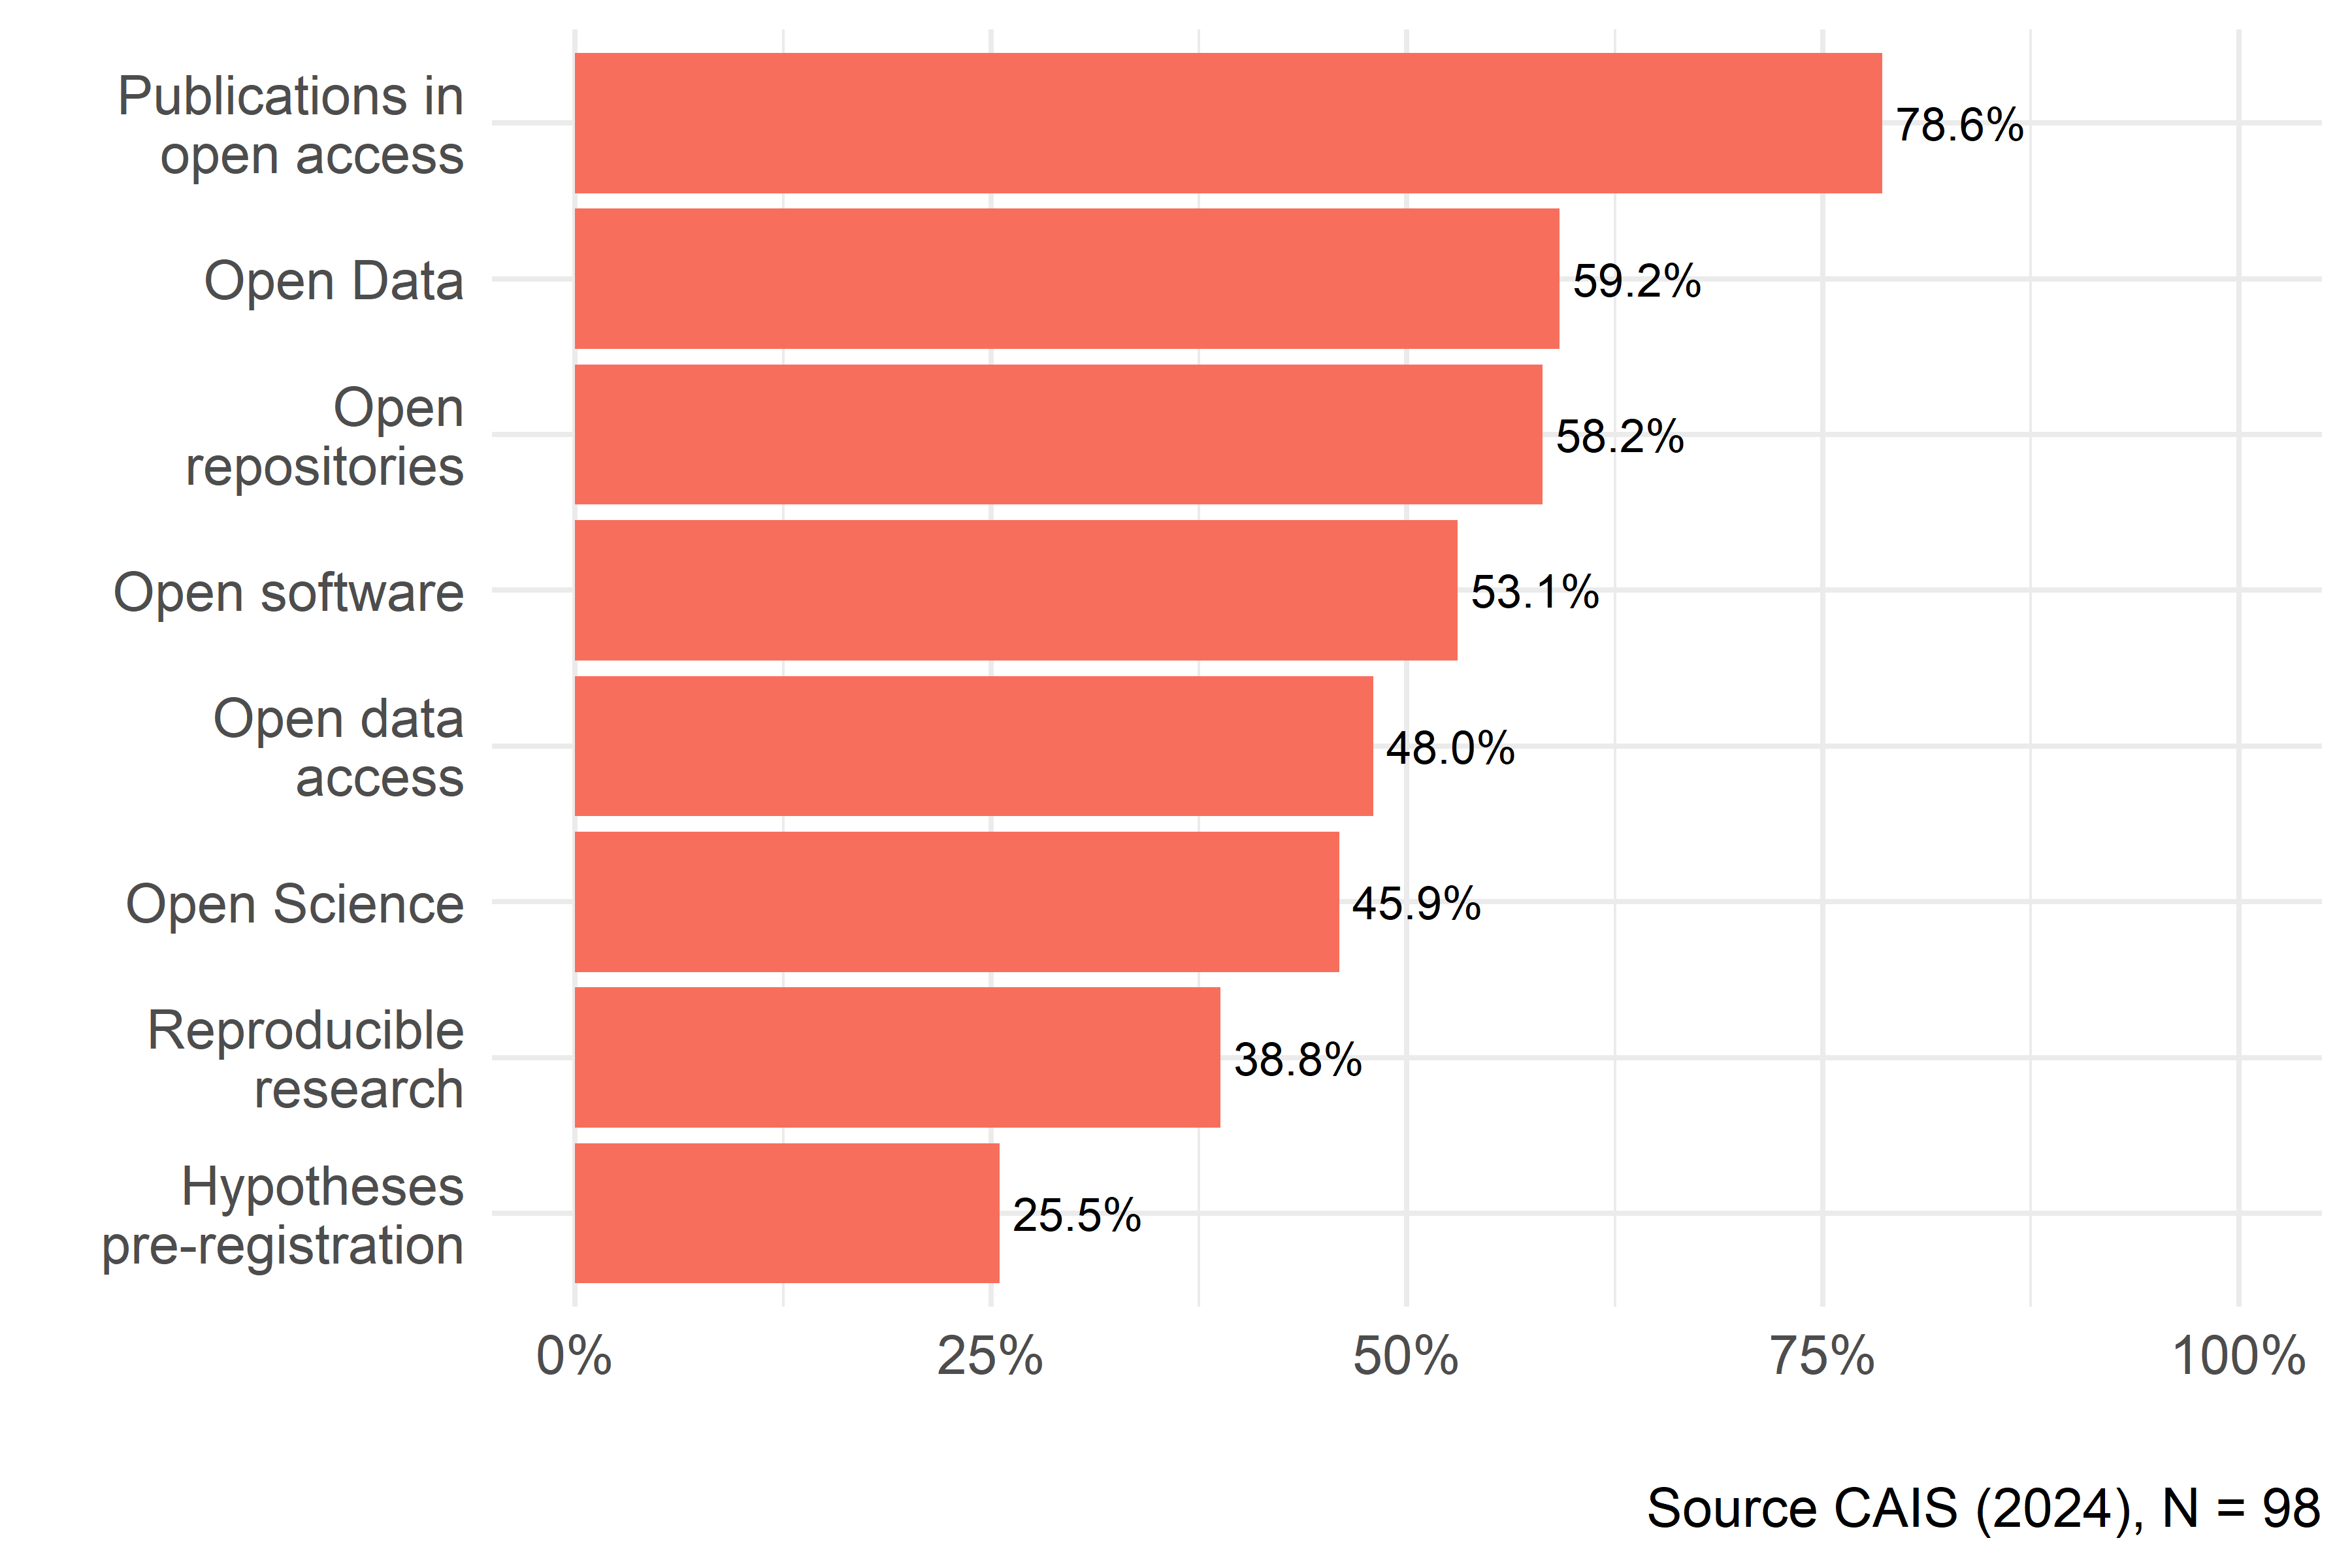
\includegraphics{paper_files/figure-pdf/fig-cca-1.png}

}

\caption{\label{fig-cca}Familiarity with Open Science concepts}

\end{figure}%

In general, knowledge levels seem to be higher among young researchers
and with a predominantly quantitative focus, as shown in the
Table~\ref{tbl-cca-grid}. Respondents between 28 and 34 years of age,
thus, show higher levels of knowledge about open software, and the
concepts of reproducible research and open science. However, researchers
between 35 and 49 years of age show higher levels of knowledge of
hypotheses preregistration and open access to data. Quantitative
researchers, meanwhile, show higher levels of knowledge of all concepts
except open access to publications.

\begin{table}

\caption{\label{tbl-cca-grid}Familiarity with Open Science concepts by
age and research strategy}

\centering{

\centering\begingroup\fontsize{9}{11}\selectfont

\resizebox{\ifdim\width>\linewidth\linewidth\else\width\fi}{!}{
\begin{tabular}[t]{>{}lllllll}
\toprule
\multicolumn{1}{c}{\textbf{ }} & \multicolumn{3}{c}{\textbf{Age group}} & \multicolumn{3}{c}{\textbf{Research strategy}} \\
\cmidrule(l{3pt}r{3pt}){2-4} \cmidrule(l{3pt}r{3pt}){5-7}
Open Science Concept & 28–34 & 35–49 & 50+ & Qualitative & Mixed & Quantitative\\
\midrule
\textbf{Open Science} & 66.7\% & 50.9\% & 29.0\% & 39.3\% & 36.1\% & 62.5\%\\
Publications in
\textbf{open access} & 83.3\% & 76.4\% & 80.6\% & 78.6\% & 83.3\% & 71.9\%\\
Hypotheses
\textbf{pre-registration} & 16.7\% & 32.7\% & 16.1\% & 3.6\% & 16.7\% & 50.0\%\\
\textbf{Open Data} & 66.7\% & 63.6\% & 48.4\% & 53.6\% & 44.4\% & 78.1\%\\
Reproducible
\textbf{research} & 58.3\% & 38.2\% & 32.3\% & 25.0\% & 30.6\% & 59.4\%\\
\addlinespace
Open
\textbf{repositories} & 58.3\% & 60.0\% & 54.8\% & 57.1\% & 52.8\% & 62.5\%\\
\textbf{Open software} & 75.0\% & 54.5\% & 41.9\% & 42.9\% & 38.9\% & 75.0\%\\
Open data
\textbf{access} & 41.7\% & 50.9\% & 45.2\% & 50.0\% & 27.8\% & 65.6\%\\
\bottomrule
\end{tabular}}
\endgroup{}

}

\end{table}%

\subsubsection{Practices}\label{practices}

\paragraph{a. Own practices and Community's
practices}\label{a.-own-practices-and-communitys-practices}

In general, the frequency of practices related to open science is low,
as seen in Figure~\ref{fig-prac}. 32\% of respondents always or almost
always use online repositories to upload information related to their
research, and 16\% report sharing code among researchers
(Figure~\ref{fig-prac-2}). These types of practices are more common
among male researchers, those whose primary research strategy is
quantitative, and those who are in an early stage in their academic
careers.

\begin{figure}

\begin{minipage}{0.50\linewidth}

\centering{

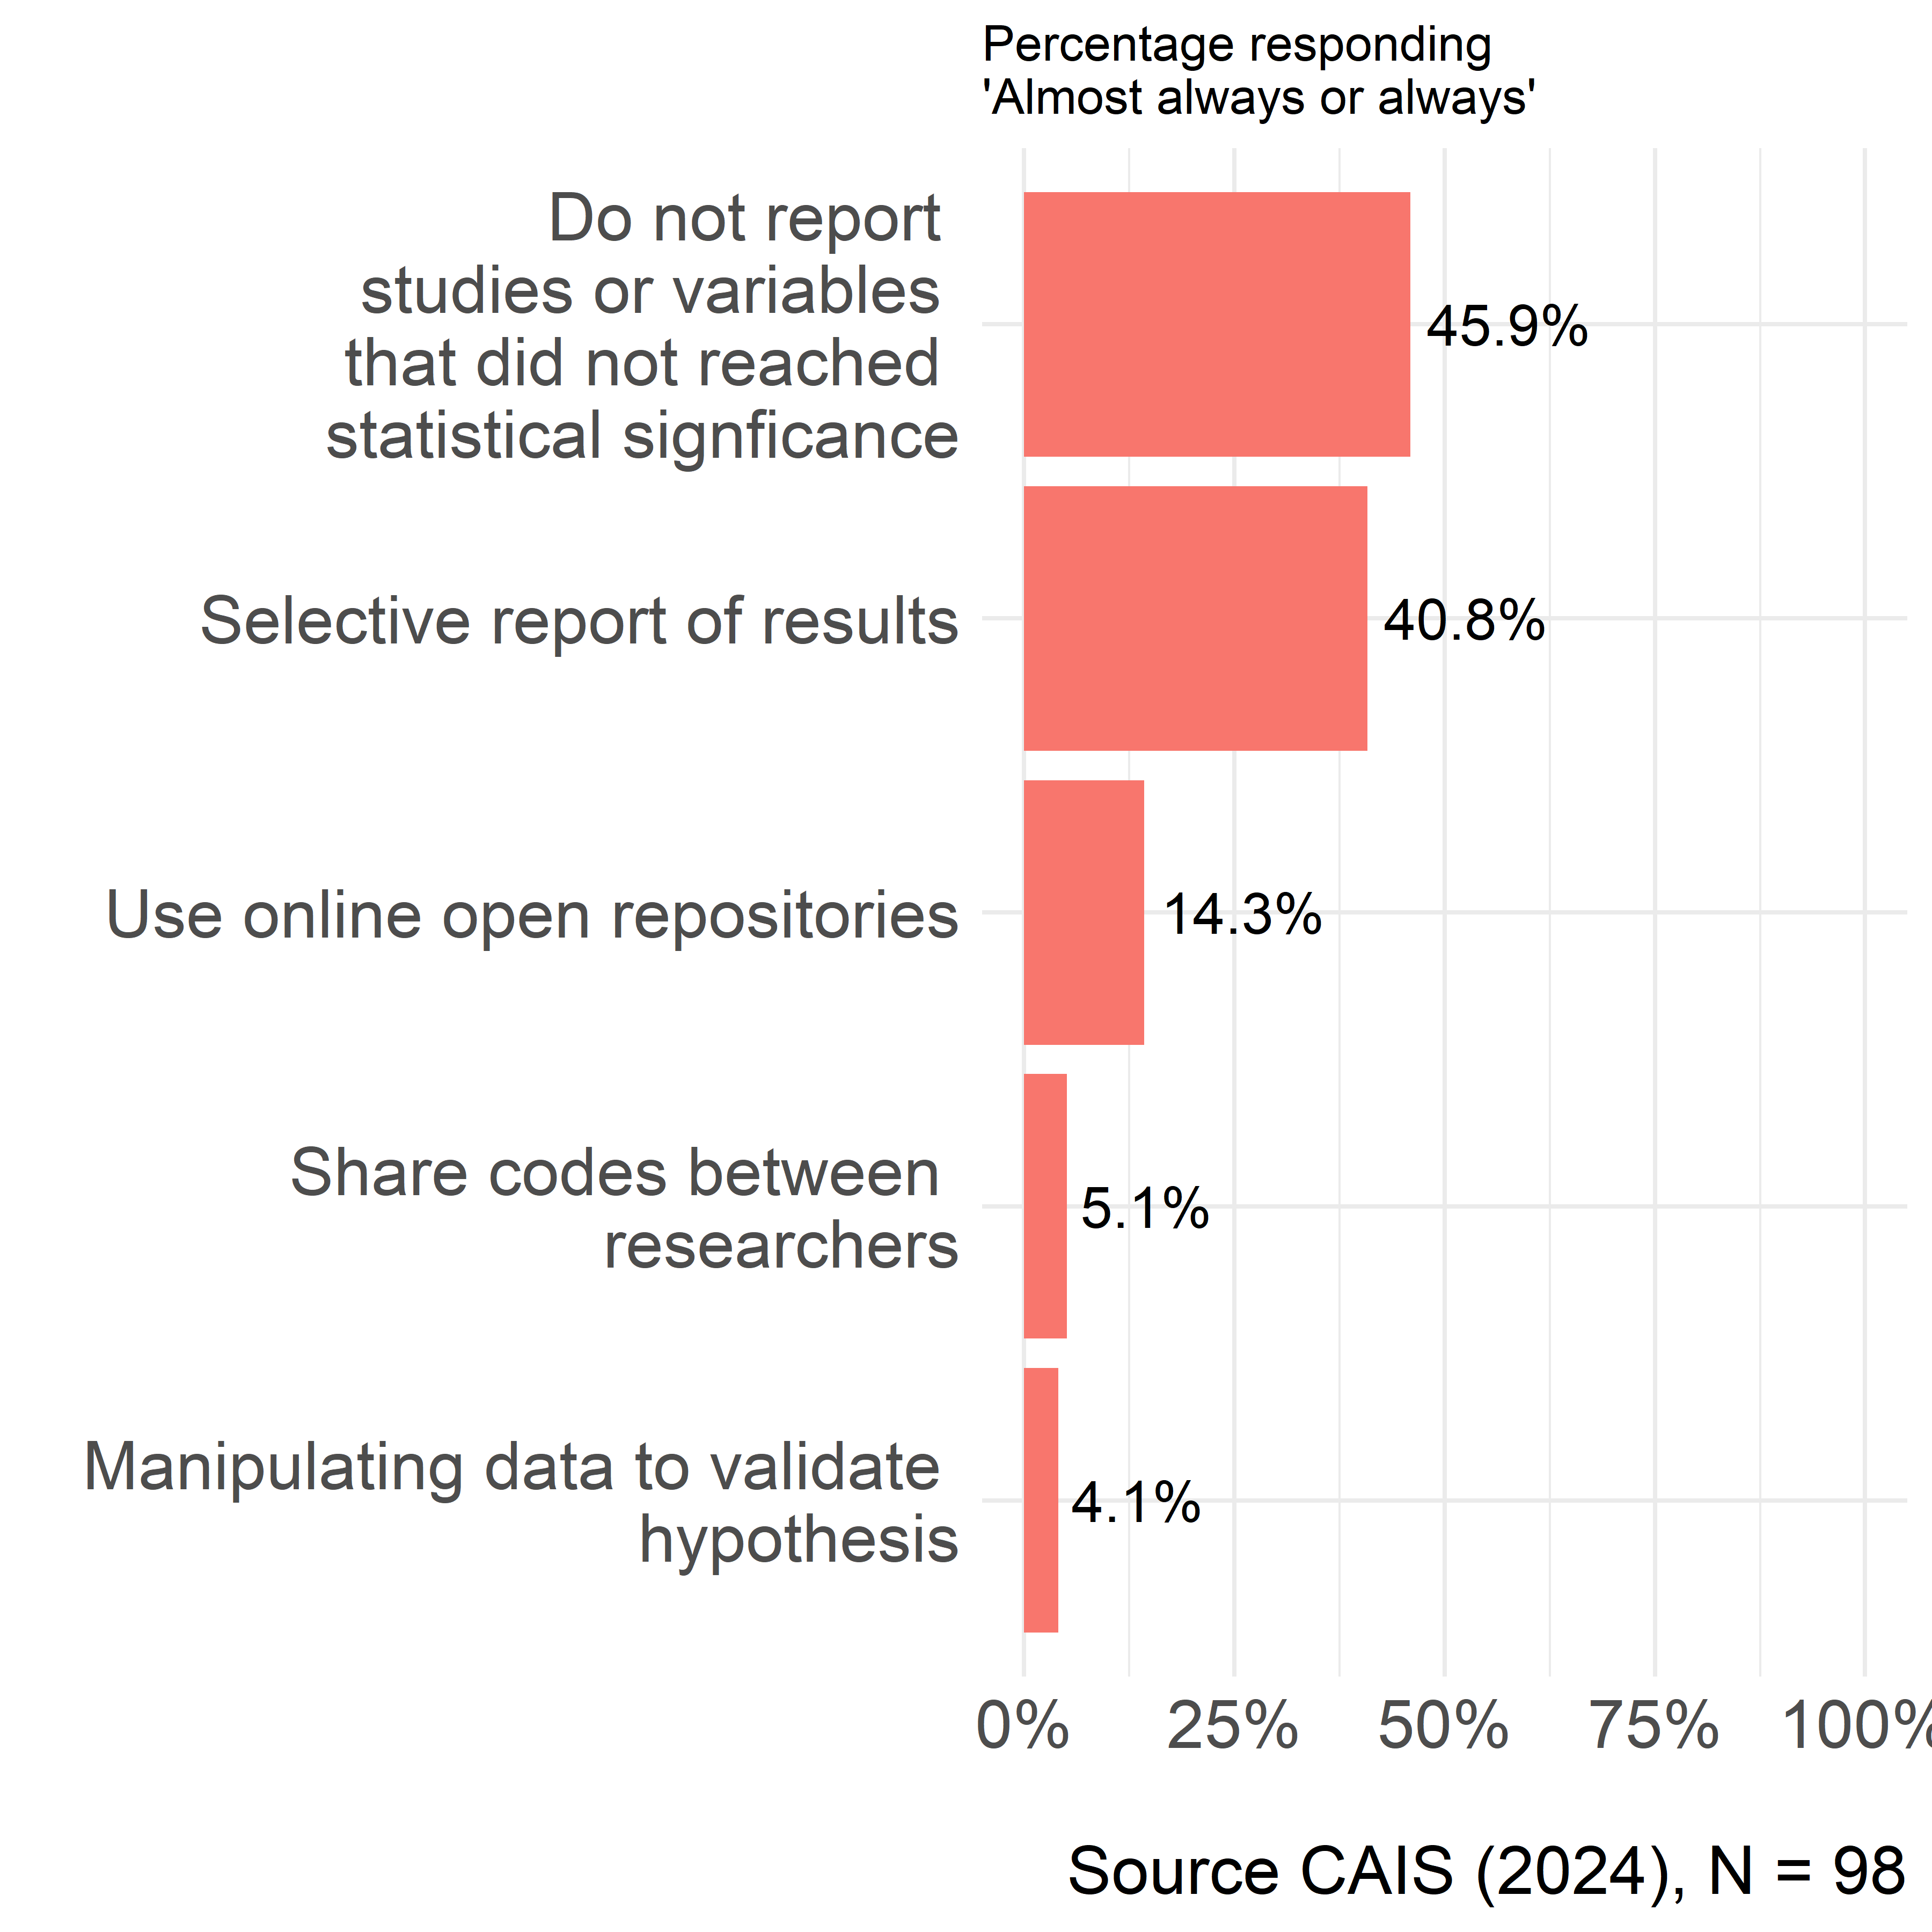
\includegraphics{paper_files/figure-pdf/fig-prac-1.png}

}

\subcaption{\label{fig-prac-1}Community's practices}

\end{minipage}%
%
\begin{minipage}{0.50\linewidth}

\centering{

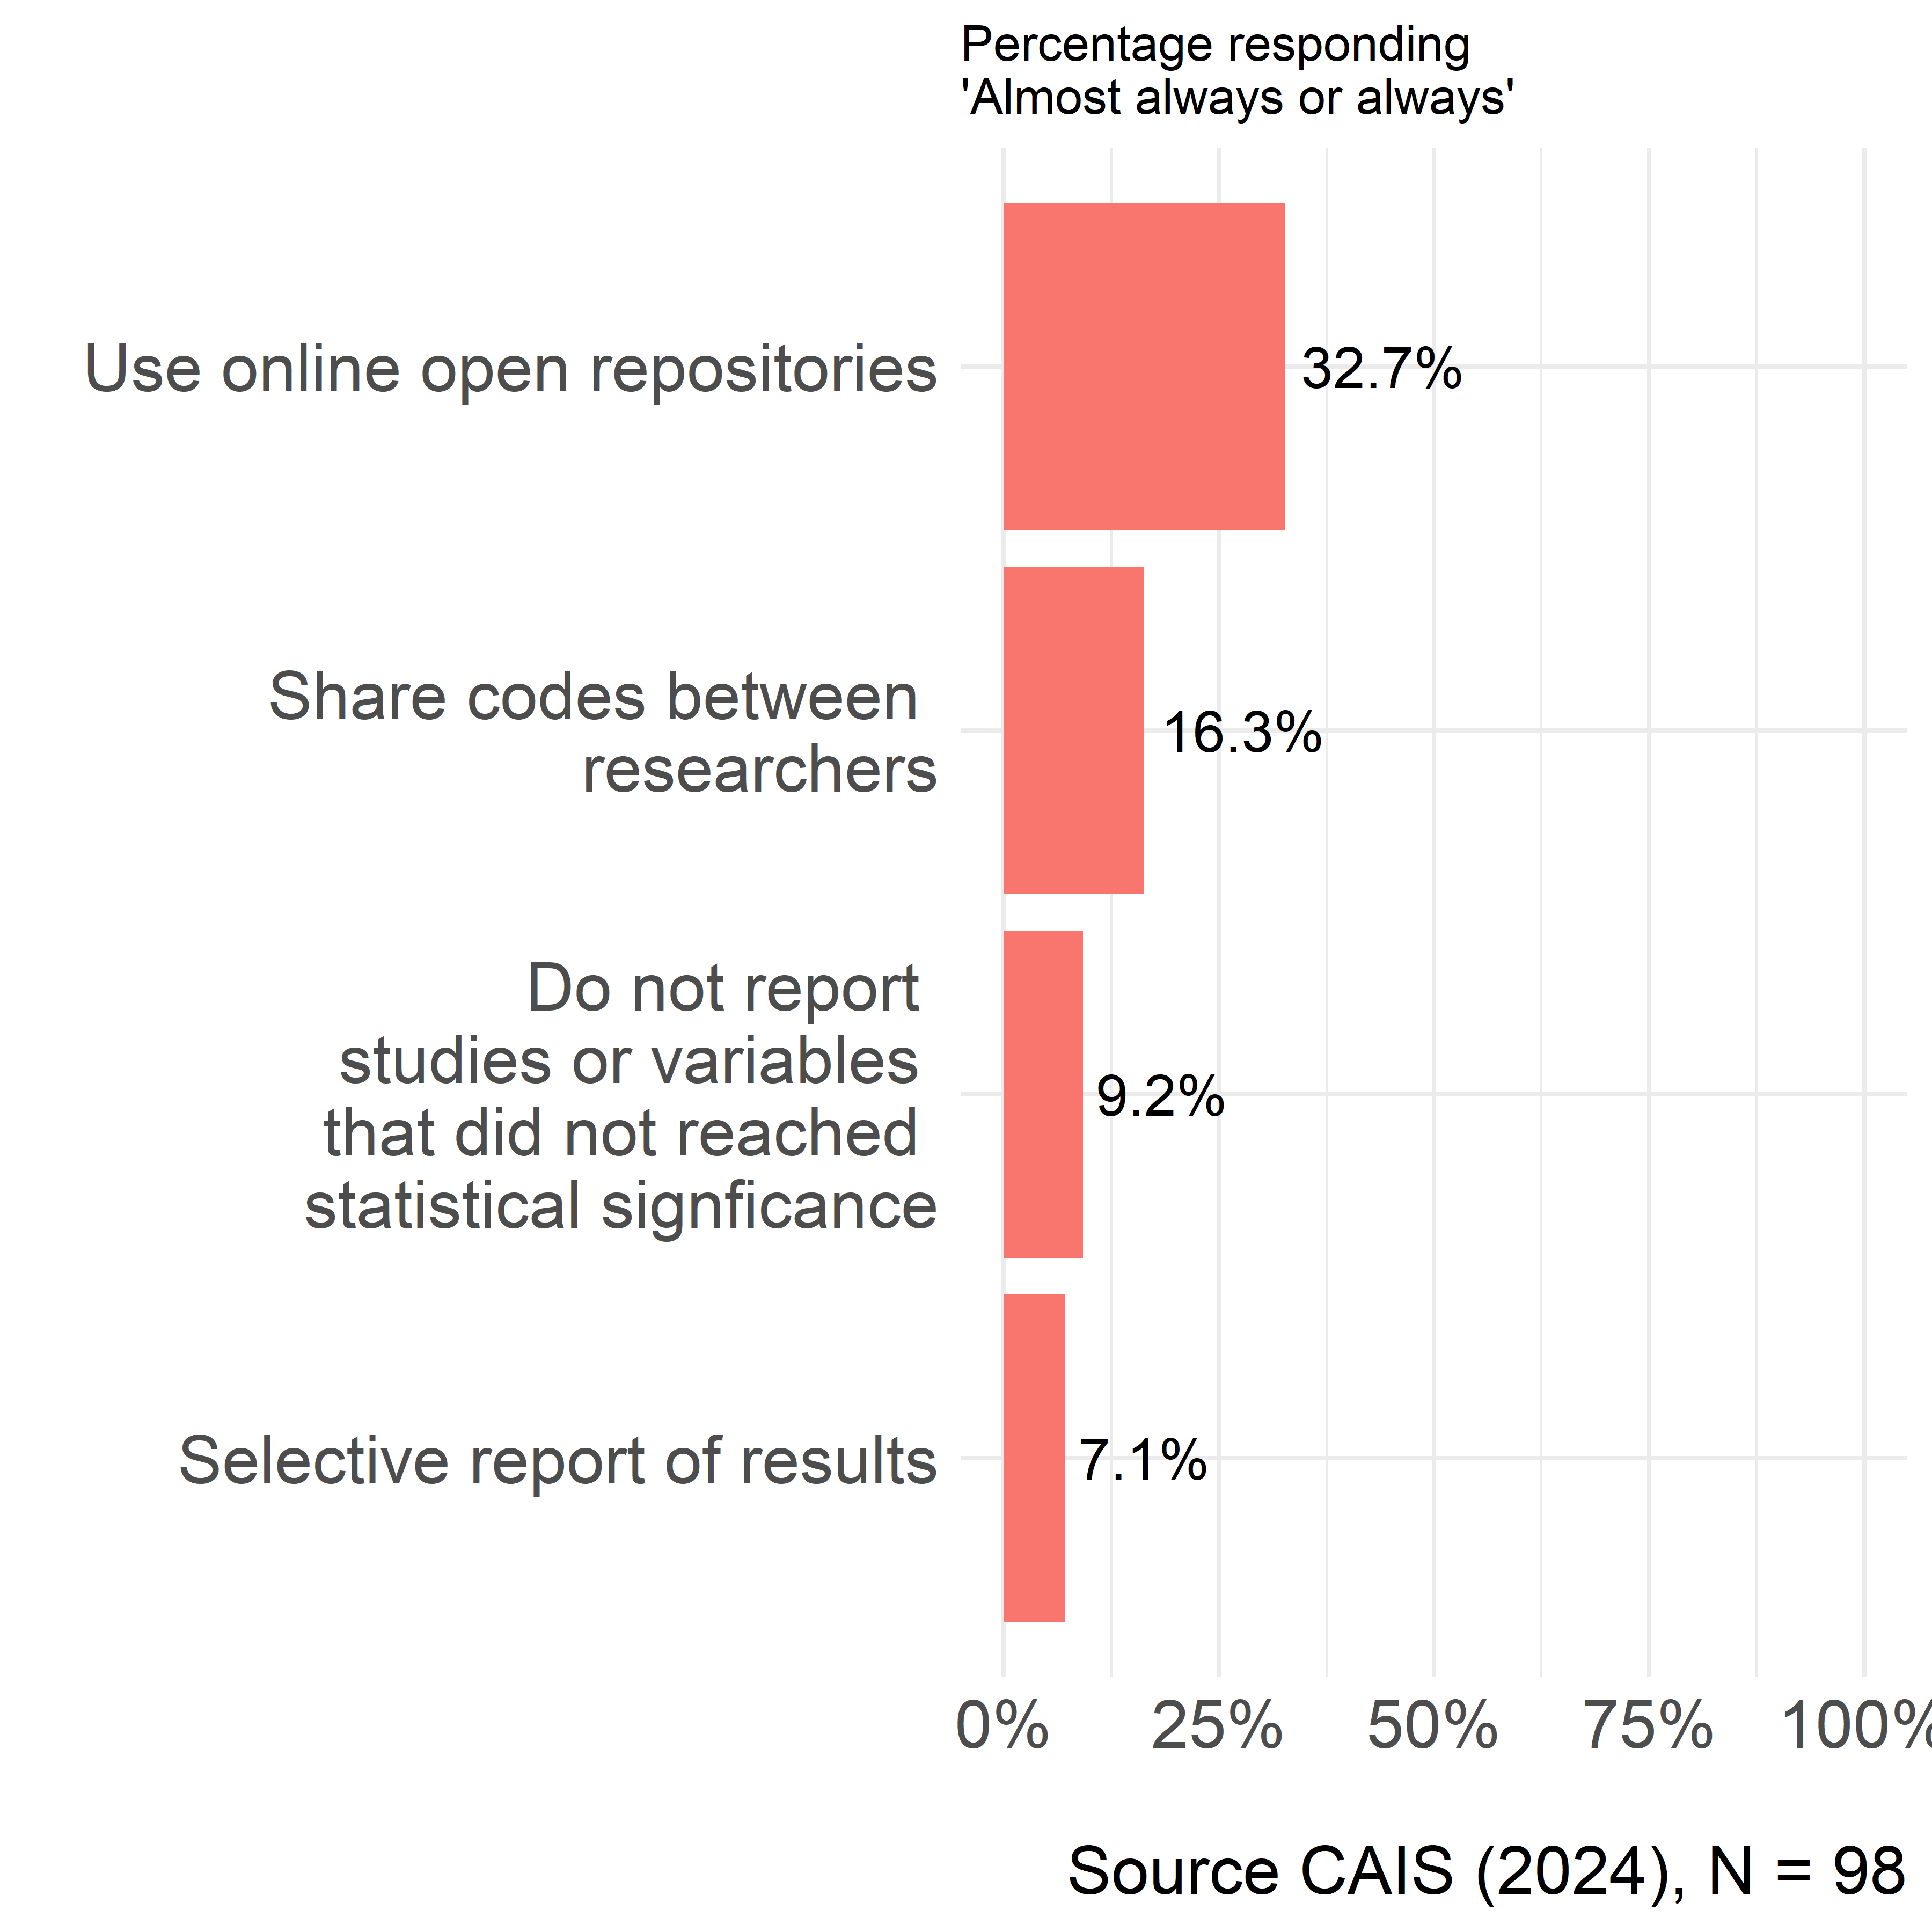
\includegraphics{paper_files/figure-pdf/fig-prac-2.png}

}

\subcaption{\label{fig-prac-2}Own Practices}

\end{minipage}%

\caption{\label{fig-prac}How often are the following practices
performed?}

\end{figure}%

Interestingly, researchers generally report better practices for
themselves than for the community. For example, only 14\% believe that
the community always or almost always uses online repositories to upload
information related to their research, and 5\% believe that researchers
share code with that frequency (Figure~\ref{fig-prac-1}).

This gap also exits in the case of malpractice. 9\% of the respondents
say they almost always or always fail to report studies or variables
that do not reach statistical significance, while 45\% believe this
practices are that common in the community. On the other hand, while 7\%
say they selectively report results, 40\% believe it is always or almost
always done in the community. Finally, while no one admits to having
manipulated data to validate a hypothesis, 4\% say this always or almost
always happens in the community.

It is curious that when the analysis is broken down into different
groups, certain trends are repeated. Male and quantitative-oriented,
researchers are at the same time those who declare the highest frequency
of own practices, both negative and positive, as well as those perceive
the highest number of negative practices in the community. These
differences can be seen in detail in the Table~\ref{tbl-prac-grid}

\begin{table}

\caption{\label{tbl-prac-grid}How often are the following practices
performed?}

\centering{

\centering\begingroup\fontsize{9}{11}\selectfont

\resizebox{\ifdim\width>\linewidth\linewidth\else\width\fi}{!}{
\begin{tabular}[t]{llllll}
\toprule
\multicolumn{1}{c}{\textbf{ }} & \multicolumn{2}{c}{\textbf{Sex}} & \multicolumn{3}{c}{\textbf{Research Strategy}} \\
\cmidrule(l{3pt}r{3pt}){2-3} \cmidrule(l{3pt}r{3pt}){4-6}
Research Practices & Women & Men & Qualitative & Mixed & Quantitative\\
\midrule
\cellcolor[HTML]{F0F0F0}{\textbf{Own practices}} & \cellcolor[HTML]{F0F0F0}{\textbf{}} & \cellcolor[HTML]{F0F0F0}{\textbf{}} & \cellcolor[HTML]{F0F0F0}{\textbf{}} & \cellcolor[HTML]{F0F0F0}{\textbf{}} & \cellcolor[HTML]{F0F0F0}{\textbf{}}\\
Share codes between 
researchers & 8.1\% & 21.3\% & NA\% & 8.3\% & 37.5\%\\
Use online open repositories & 24.3\% & 37.7\% & 21.4\% & 25.0\% & 46.9\%\\
Selective report of results & 2.7\% & 9.8\% & 3.6\% & 5.6\% & 12.5\%\\
Do not report 
studies or variables 
 that did not reached 
statistical signficance & 8.1\% & 9.8\% & 3.6\% & 11.1\% & 12.5\%\\
\addlinespace
\cellcolor[HTML]{F0F0F0}{\textbf{Community's practices}} & \cellcolor[HTML]{F0F0F0}{\textbf{}} & \cellcolor[HTML]{F0F0F0}{\textbf{}} & \cellcolor[HTML]{F0F0F0}{\textbf{}} & \cellcolor[HTML]{F0F0F0}{\textbf{}} & \cellcolor[HTML]{F0F0F0}{\textbf{}}\\
Share codes between 
researchers & 8.1\% & 3.3\% & 3.6\% & 5.6\% & 6.2\%\\
Use online open repositories & 18.9\% & 11.5\% & 14.3\% & 13.9\% & 12.5\%\\
Selective report of results & 27.0\% & 49.2\% & 17.9\% & 50.0\% & 50.0\%\\
Do not report 
studies or variables 
 that did not reached 
statistical signficance & 29.7\% & 55.7\% & 25.0\% & 55.6\% & 50.0\%\\
\addlinespace
Manipulating data to validate 
hypothesis & 2.7\% & 4.9\% & 7.1\% & 2.8\% & 3.1\%\\
\bottomrule
\end{tabular}}
\endgroup{}

}

\end{table}%

\paragraph{b. Open Science Barriers}\label{b.-open-science-barriers}

There is a high perception of barriers to the development of Open
Science in all its dimensions. Lack of policy is perceived as the main
barrier in all dimensions, as can be seen in the
Figure~\ref{fig-barreras}. Lacks of knowledge also appears as a major
barrier especially for transparent design, open data and reproducible
research. Finally, lack of incentives is recognized as another aspect
that hinders data openness.

\begin{figure}

\centering{

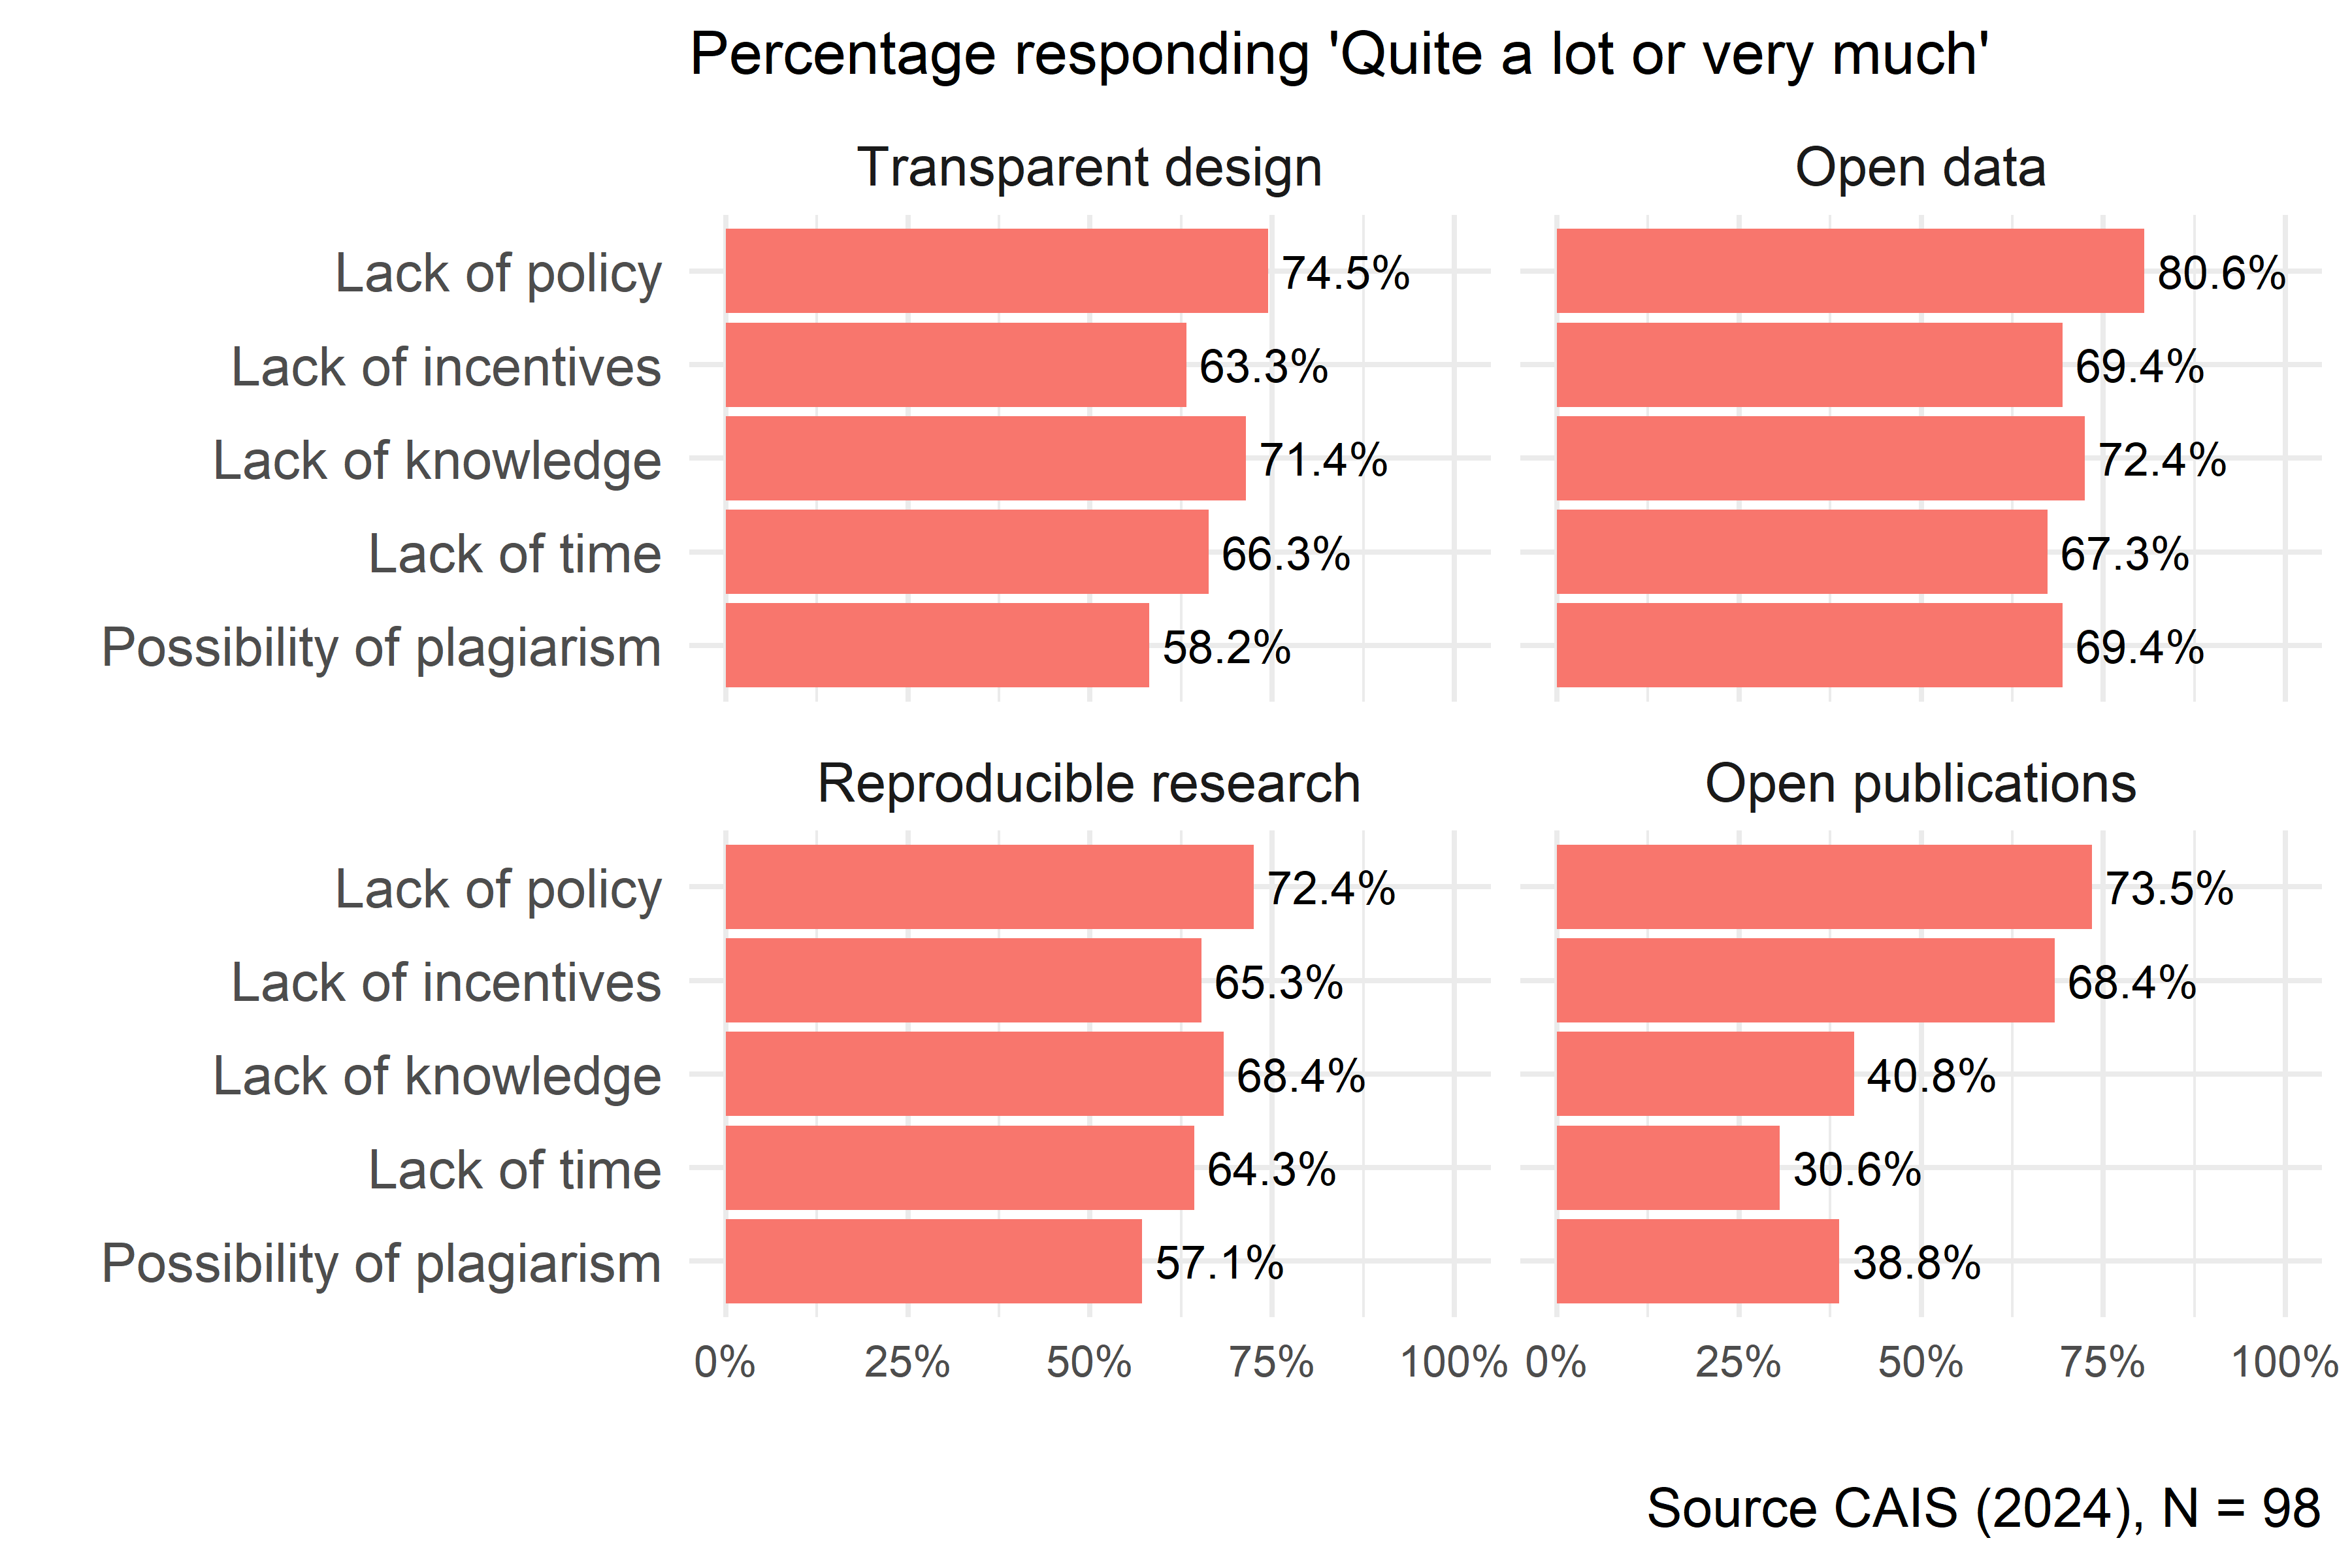
\includegraphics{paper_files/figure-pdf/fig-barreras-1.png}

}

\caption{\label{fig-barreras}¿To what extent do you consider that the
following factors limit Open Science?}

\end{figure}%

Regarding this last point, the incentives that researchers might have to
open their data were analyzed. As can be seen in the
Figure~\ref{fig-motivaciones}, networking, the dissemination of publicly
funded data to the community, and the increase of one's own visibility
are highly valued as incentives for open data.

\begin{figure}

\centering{

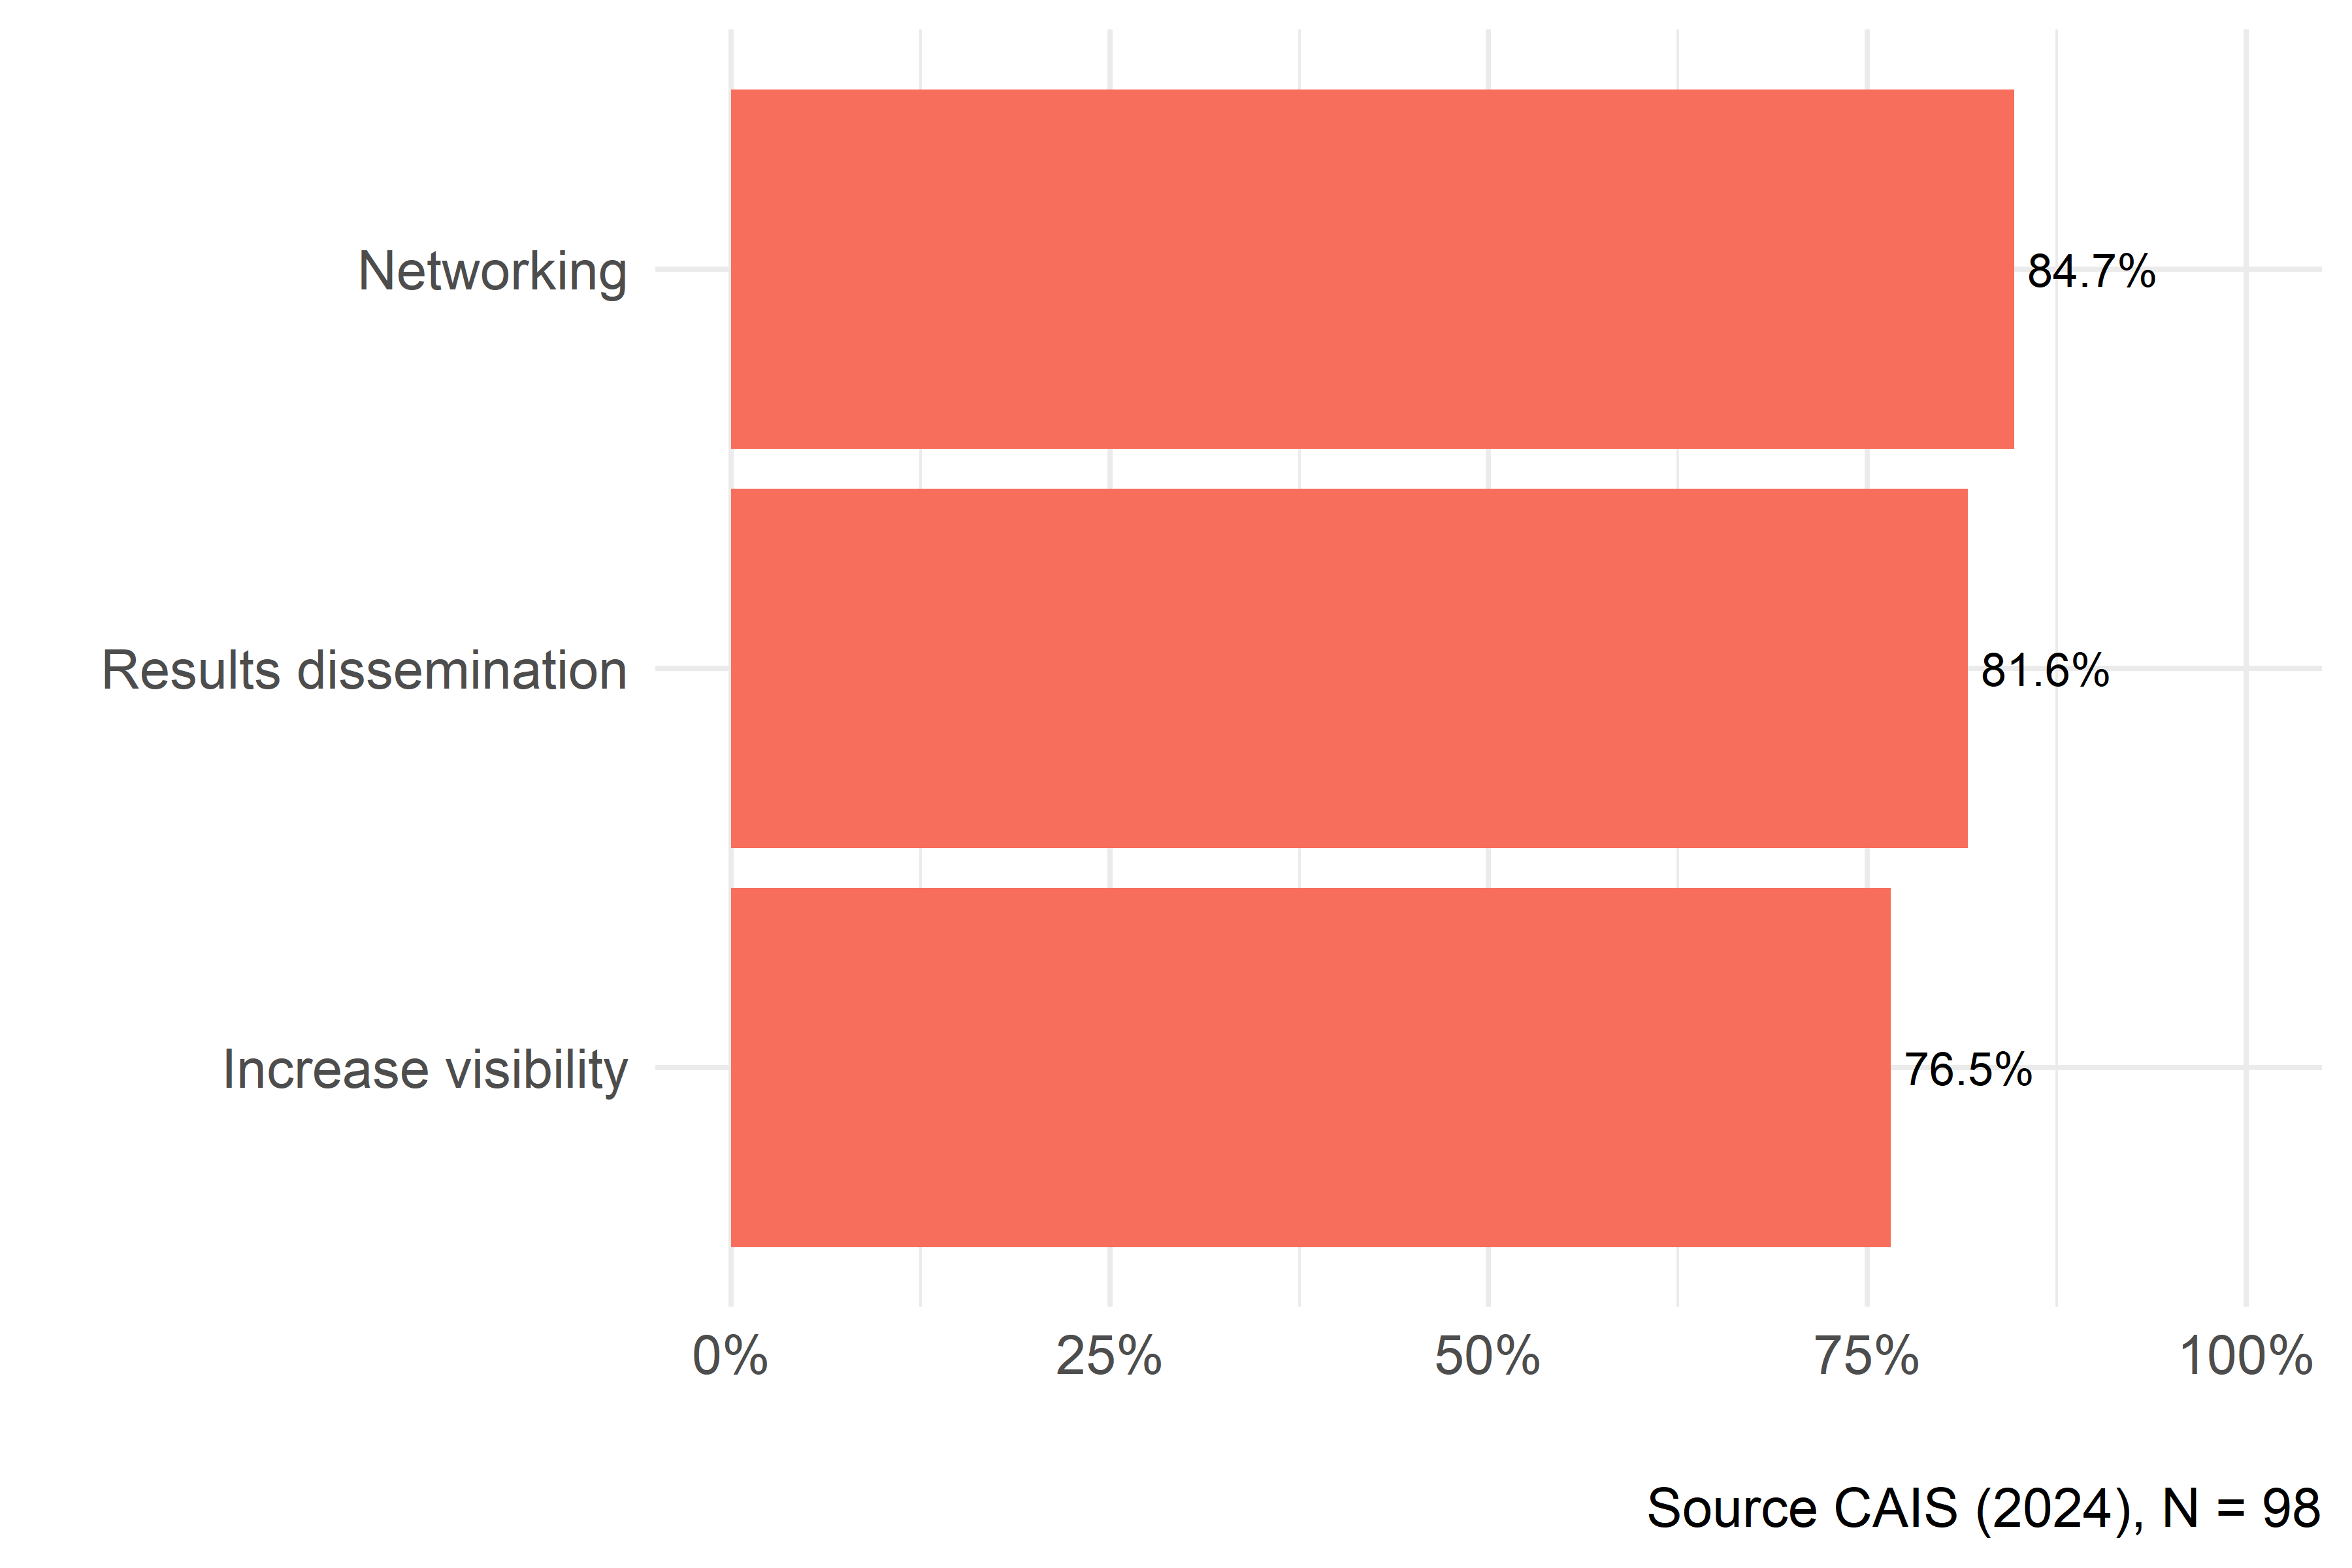
\includegraphics{paper_files/figure-pdf/fig-motivaciones-1.png}

}

\caption{\label{fig-motivaciones}Open data motivations}

\end{figure}%

\subsubsection{Attitudes}\label{attitudes}

\paragraph{a. Attitudes on Open Science
Measures}\label{a.-attitudes-on-open-science-measures}

In general, the possibility of adopting Open Science measures in the
social sciences is assessed positively, as can be see in
Figure~\ref{fig-val}. Open access (92\%), replication of results (67\%),
reporting of non-statistically significant results (76\%), and online
availability of data and analysis materials (72\%) all show a high level
of acceptance among respondents. The only exception is the
pre-registration of hypothesis, which received a positive evaluation of
only 42\%. This is explained by a higher level of unfamiliarity (17\%
say they are not aware of the measure), in addition to the reluctance
already observed in the qualitative study.

\begin{figure}

\centering{

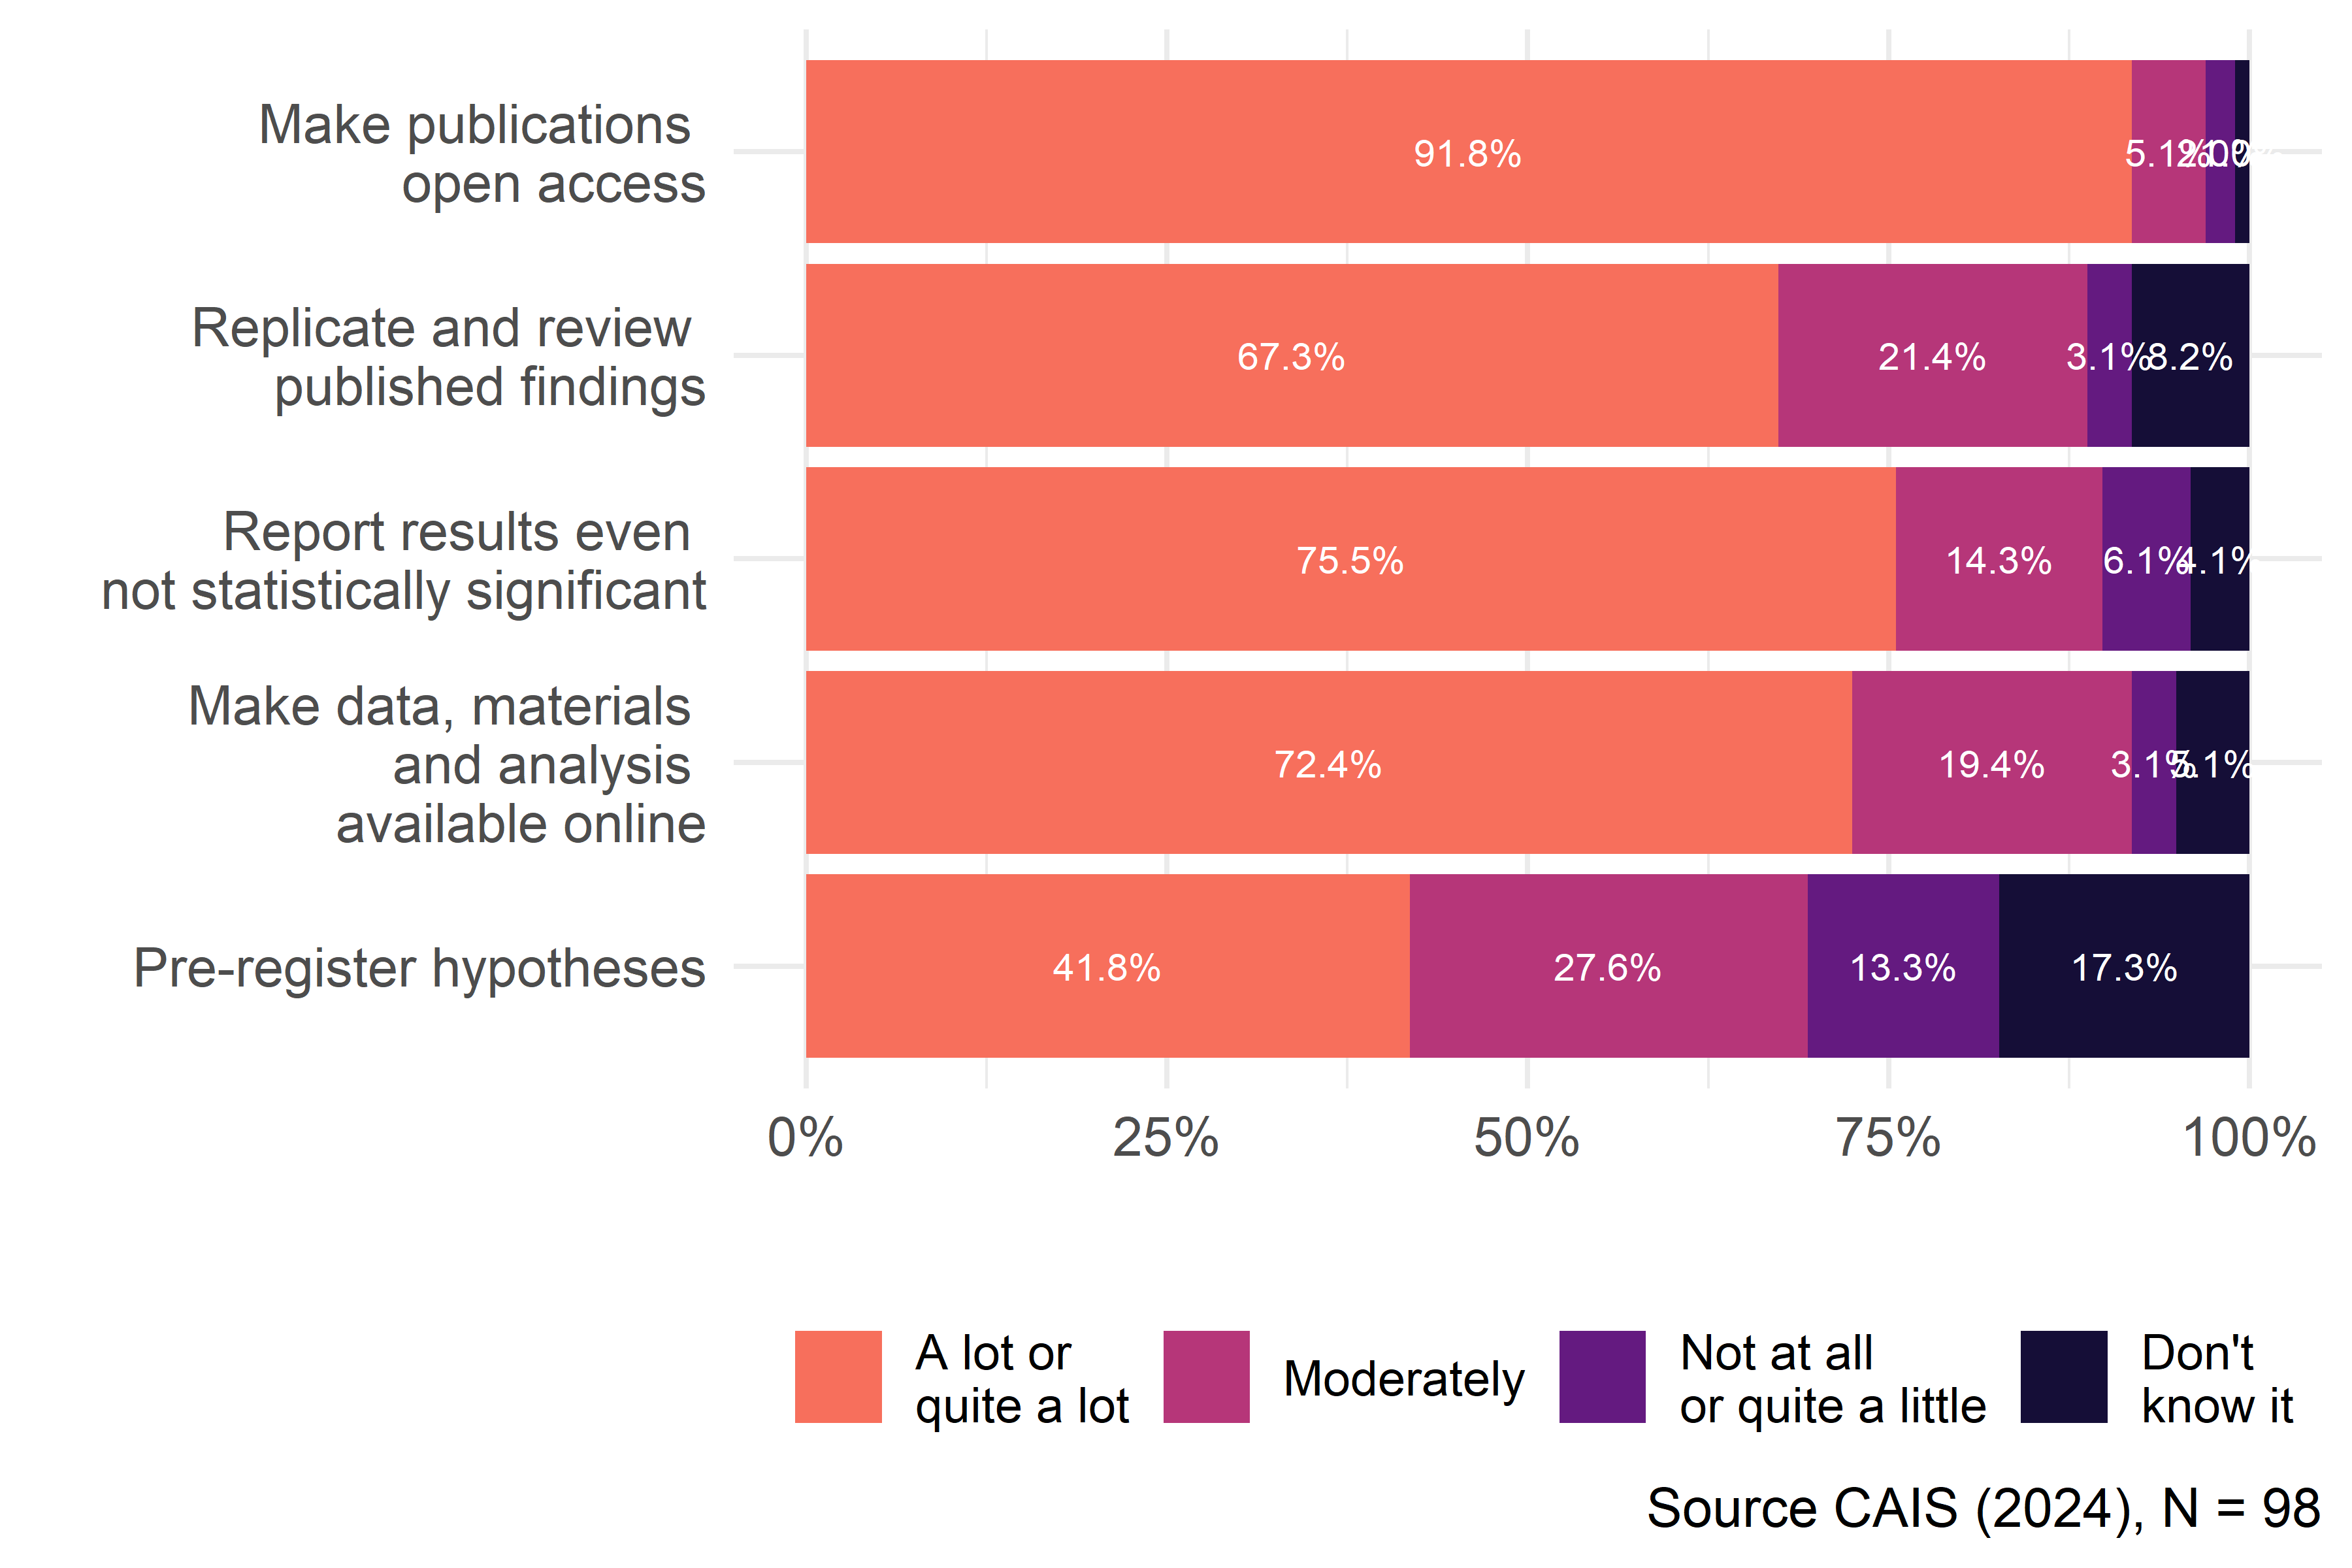
\includegraphics{paper_files/figure-pdf/fig-val-1.png}

}

\caption{\label{fig-val}How necessary do you think the following Open
Science measure are for social science research?}

\end{figure}%

\paragraph{b. Attitudes about the Replication
Crisis}\label{b.-attitudes-about-the-replication-crisis}

As shown in the Figure~\ref{fig-dona}, 39\% of respondents believe there
is a major replication crisis, while 40\% do not know if there is one.
Concern is greater among quantitative researchers, as seen in
Figure~\ref{fig-dona-grid}, with 70\% believing that the crisis is
important. While there is no denial of the crisis among qualitative
researchers, 60\% do not know if there is a crisis or not.

\begin{figure}

\centering{

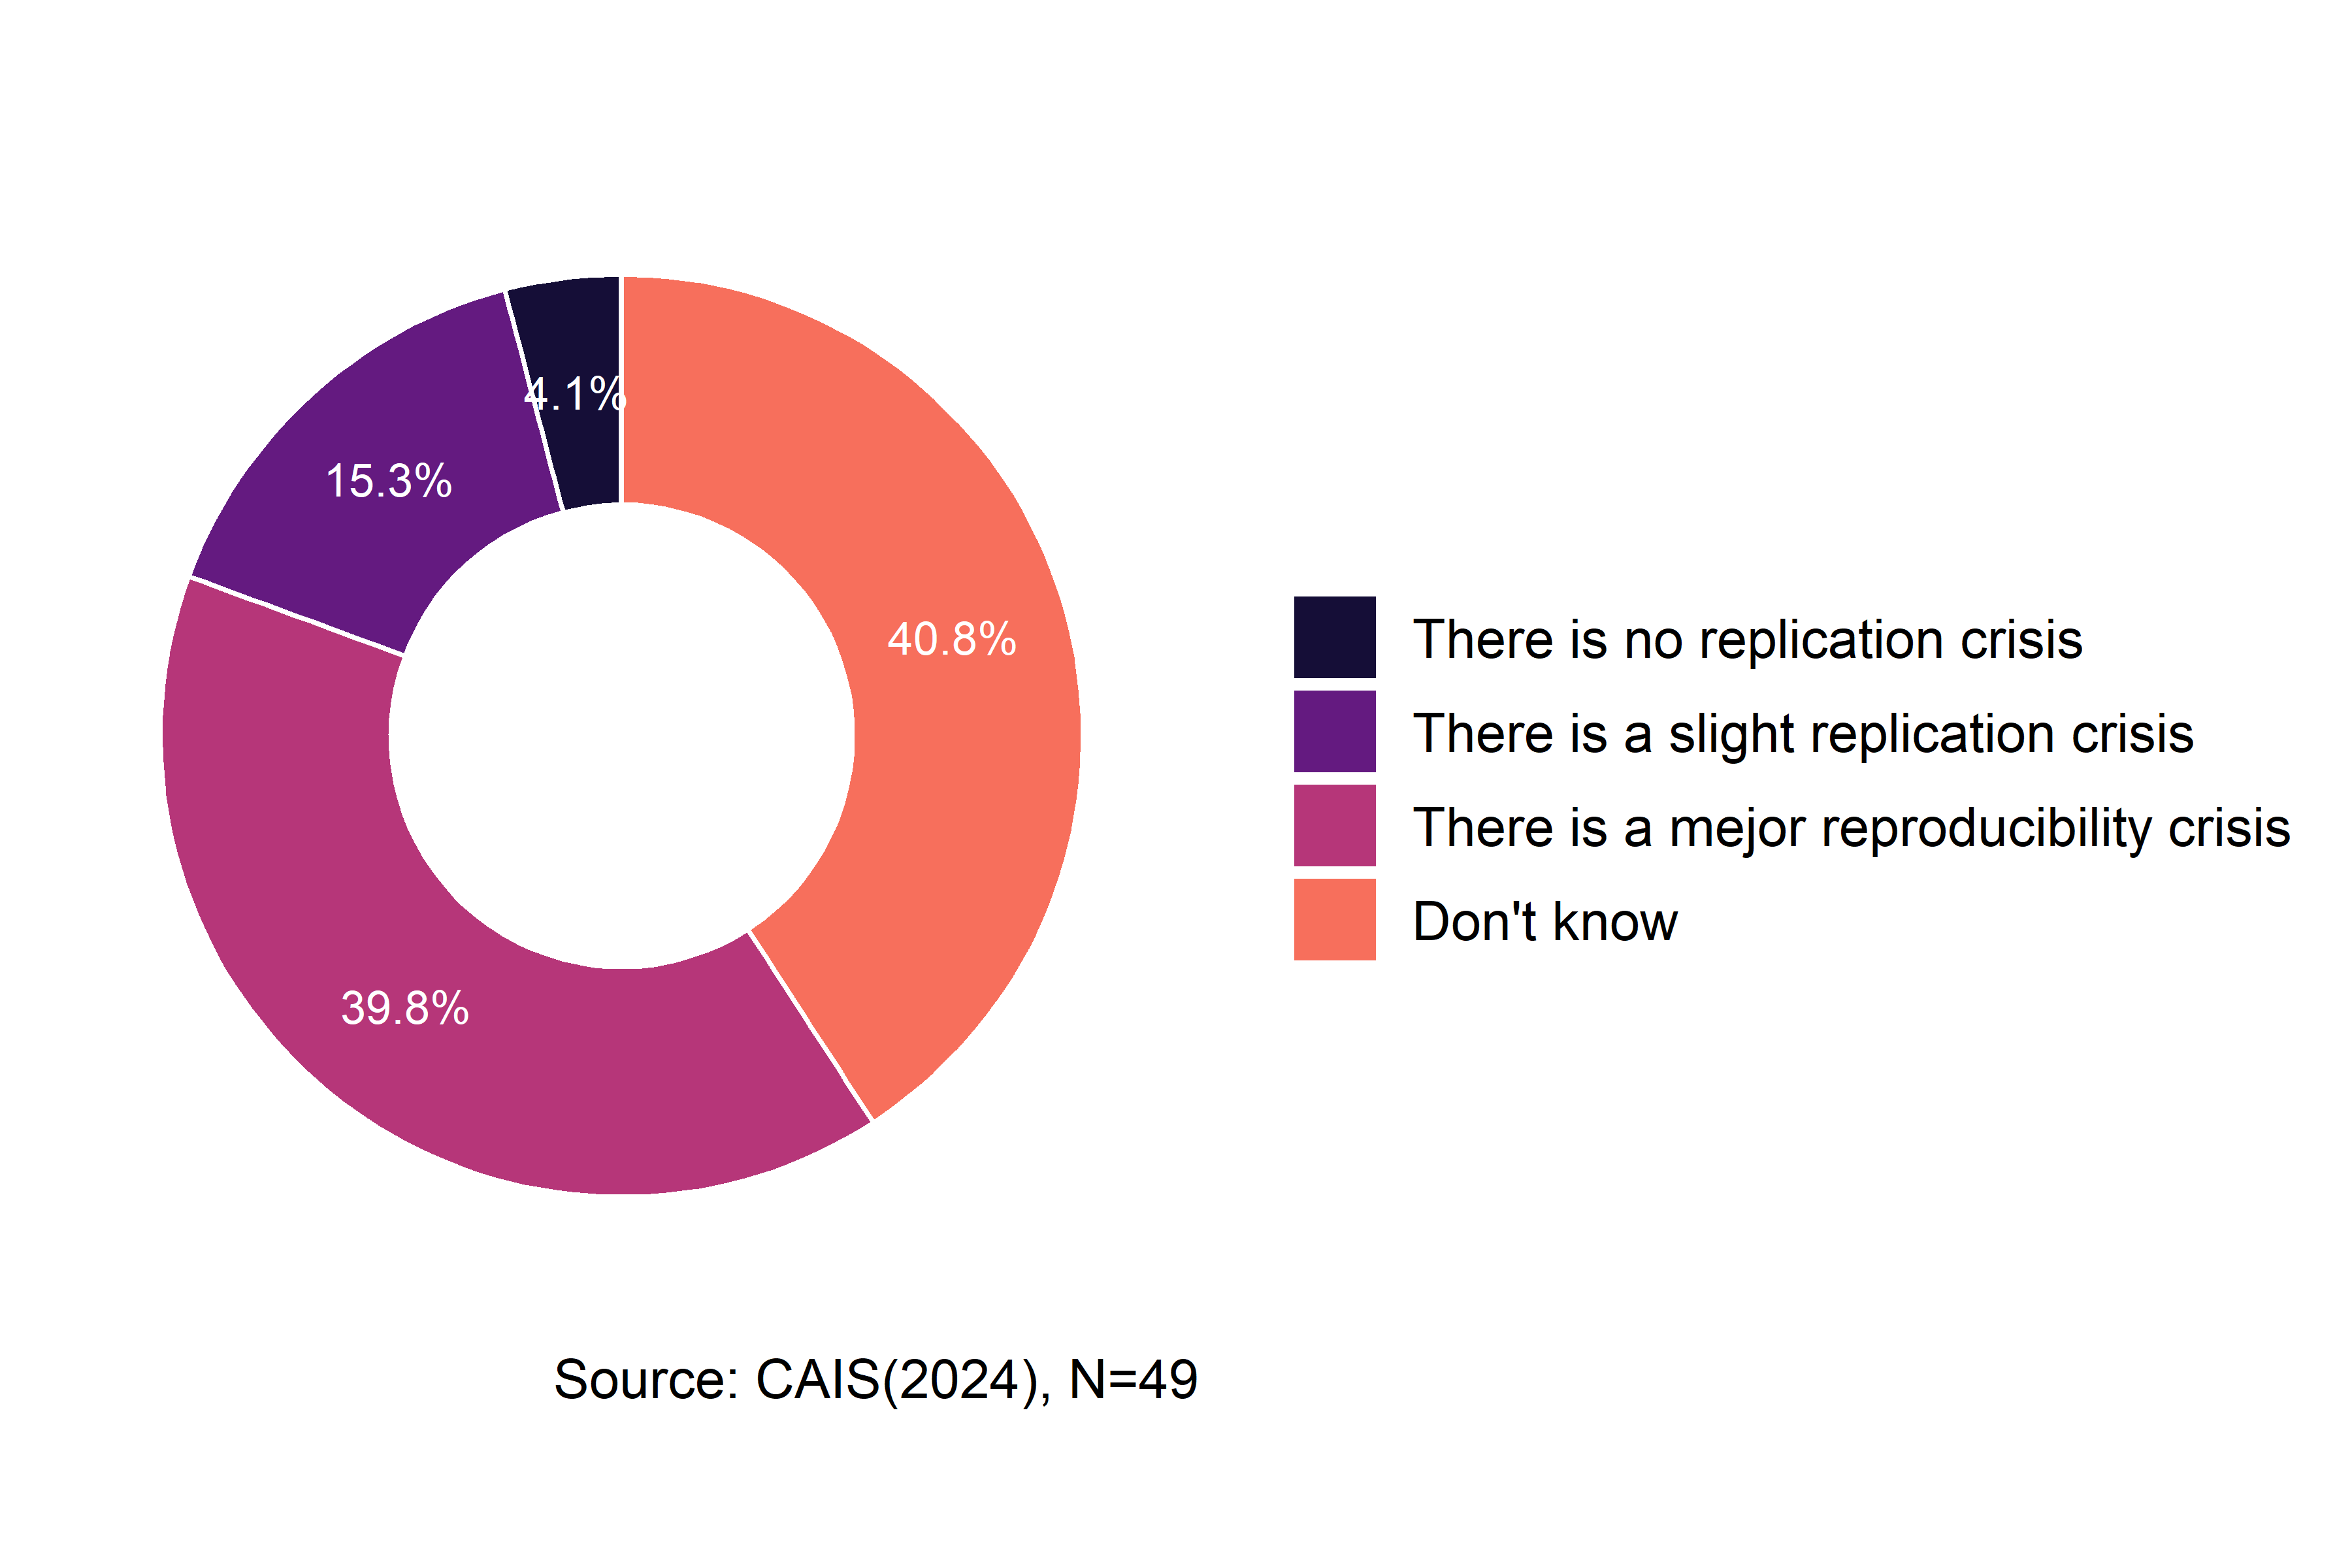
\includegraphics{paper_files/figure-pdf/fig-dona-1.png}

}

\caption{\label{fig-dona}With which of the following statement regarding
the replication crisis do you agree?}

\end{figure}%

\begin{figure}

\centering{

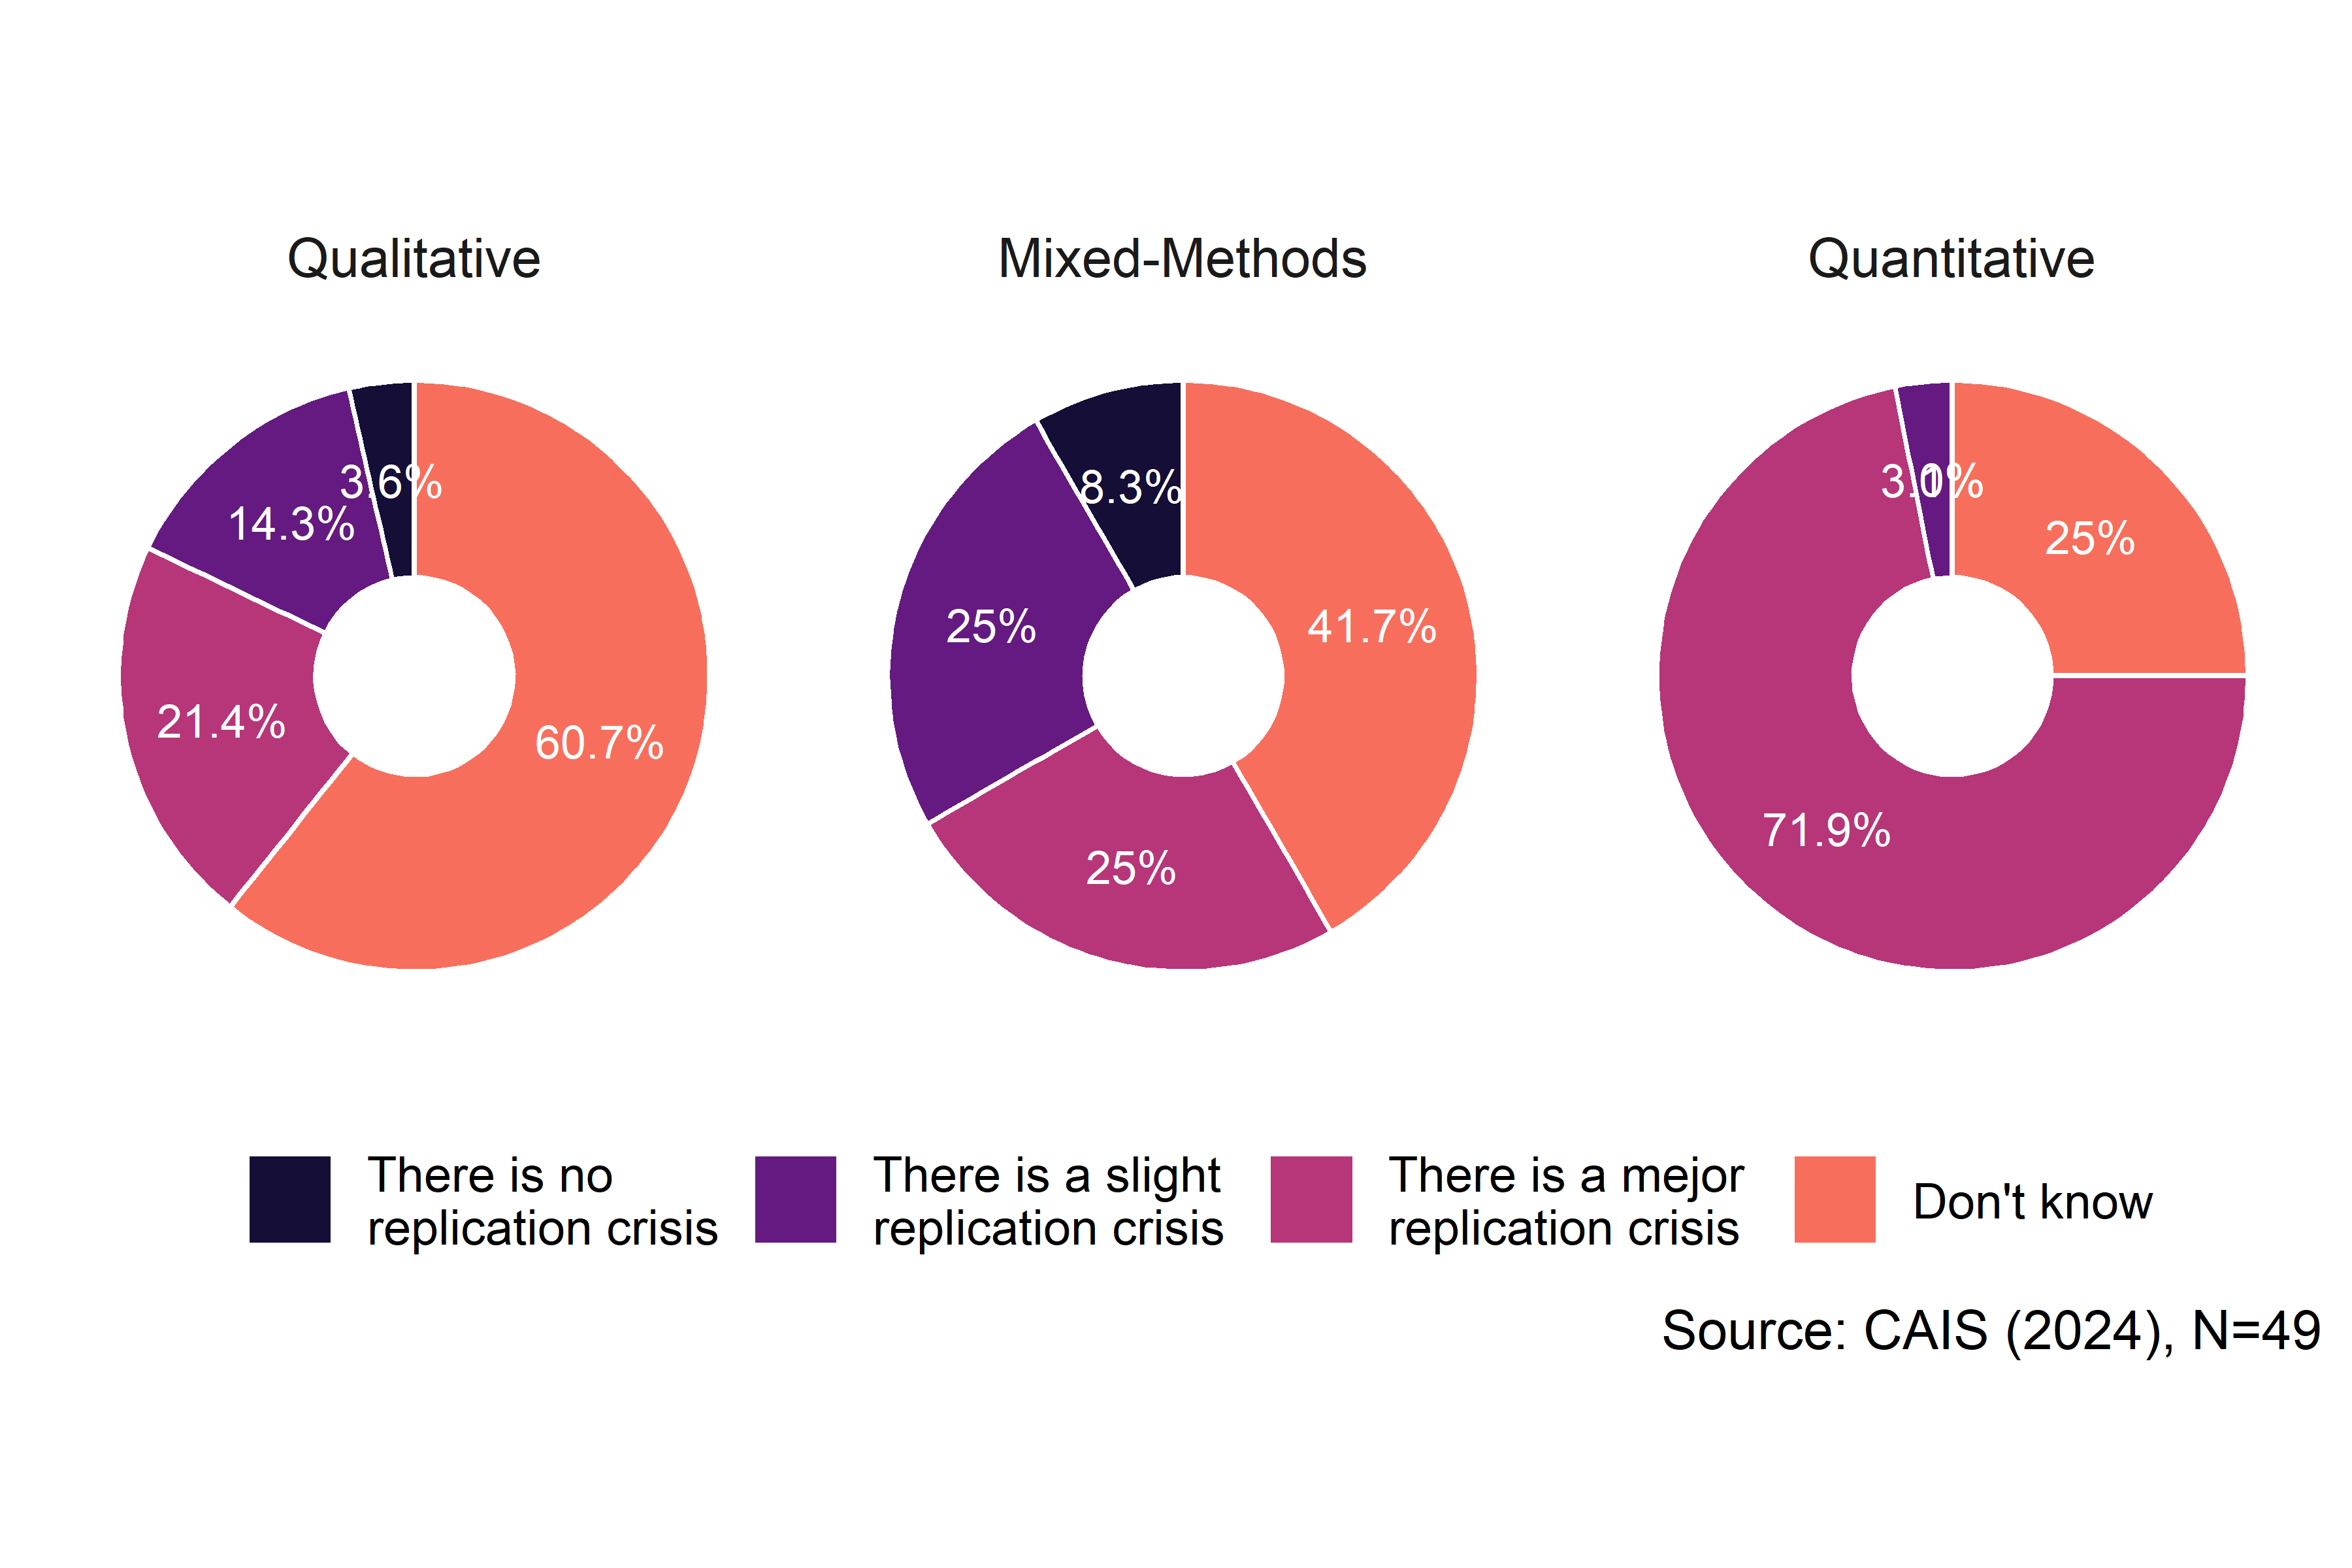
\includegraphics{paper_files/figure-pdf/fig-dona-grid-1.png}

}

\caption{\label{fig-dona-grid}Perception of the reproducibility crisis
by research strategy.}

\end{figure}%

\paragraph{c.~Attidues about ANID's Open Science
policies}\label{c.-attidues-about-anids-open-science-policies}

In the first instance, ANID's Open Science Policy is well received by
the respondents. For example, 89.7\% agree or strongly agree that ANID
should continue to develop its Open Science Policy, as show in
Table~\ref{tbl-anid}. Similarly, 83.5\% consider the implementation of
Open Access policies to be quite or very necessary.

\begin{longtable}[]{@{}
  >{\raggedright\arraybackslash}p{(\columnwidth - 6\tabcolsep) * \real{0.4019}}
  >{\raggedright\arraybackslash}p{(\columnwidth - 6\tabcolsep) * \real{0.3084}}
  >{\raggedright\arraybackslash}p{(\columnwidth - 6\tabcolsep) * \real{0.1963}}
  >{\raggedright\arraybackslash}p{(\columnwidth - 6\tabcolsep) * \real{0.0935}}@{}}
\caption{Attidues about ANID's Open Science
policies}\label{tbl-anid}\tabularnewline
\toprule\noalign{}
\begin{minipage}[b]{\linewidth}\raggedright
Variable
\end{minipage} & \begin{minipage}[b]{\linewidth}\raggedright
Stats / Values
\end{minipage} & \begin{minipage}[b]{\linewidth}\raggedright
Freqs (\% of Valid)
\end{minipage} & \begin{minipage}[b]{\linewidth}\raggedright
Valid
\end{minipage} \\
\midrule\noalign{}
\endfirsthead
\toprule\noalign{}
\begin{minipage}[b]{\linewidth}\raggedright
Variable
\end{minipage} & \begin{minipage}[b]{\linewidth}\raggedright
Stats / Values
\end{minipage} & \begin{minipage}[b]{\linewidth}\raggedright
Freqs (\% of Valid)
\end{minipage} & \begin{minipage}[b]{\linewidth}\raggedright
Valid
\end{minipage} \\
\midrule\noalign{}
\endhead
\bottomrule\noalign{}
\endlastfoot
\begin{minipage}[t]{\linewidth}\raggedright
How much do you agree with ANID continuing to develop and implement open
access policies for scientific production?\\
{[}factor{]}\strut
\end{minipage} & \begin{minipage}[t]{\linewidth}\raggedright
1. Strongly Disagree\\
2. Disagree\\
3. Neither Agree nor Disagre\\
4. Agree\\
5. Strongly Agree\strut
\end{minipage} & \begin{minipage}[t]{\linewidth}\raggedright
2 ( 2.1\%)\\
2 ( 2.1\%)\\
6 ( 6.2\%)\\
32 (33.0\%)\\
55 (56.7\%)\strut
\end{minipage} & \begin{minipage}[t]{\linewidth}\raggedright
97\\
(99.0\%)\strut
\end{minipage} \\
\begin{minipage}[t]{\linewidth}\raggedright
How necessary is the implementation of mandatory open access policies
for publicly funded research?\\
{[}factor{]}\strut
\end{minipage} & \begin{minipage}[t]{\linewidth}\raggedright
1. Not necessary at all\\
2. Slightly necessary\\
3. Moderately necessary\\
4. Quite necessary\\
5. Very necessary\strut
\end{minipage} & \begin{minipage}[t]{\linewidth}\raggedright
2 ( 2.1\%)\\
4 ( 4.1\%)\\
10 (10.3\%)\\
40 (41.2\%)\\
41 (42.3\%)\strut
\end{minipage} & \begin{minipage}[t]{\linewidth}\raggedright
97\\
(99.0\%)\strut
\end{minipage} \\
\begin{minipage}[t]{\linewidth}\raggedright
How neccesary is it for ANID to incorporate pre-registration of research
design within its Open Access Policy?\\
{[}factor{]}\strut
\end{minipage} & \begin{minipage}[t]{\linewidth}\raggedright
1. Not necessary at all\\
2. Slightly necessary\\
3. Moderately necessary\\
4. Quite necessary\\
5. Very necessary\strut
\end{minipage} & \begin{minipage}[t]{\linewidth}\raggedright
5 (10.2\%)\\
6 (12.2\%)\\
14 (28.6\%)\\
18 (36.7\%)\\
6 (12.2\%)\strut
\end{minipage} & \begin{minipage}[t]{\linewidth}\raggedright
49\\
(50.0\%)\strut
\end{minipage} \\
\begin{minipage}[t]{\linewidth}\raggedright
How neccesary is it for ANID to incorporate reproducibility of research
within its Open Access Policy\\
{[}factor{]}\strut
\end{minipage} & \begin{minipage}[t]{\linewidth}\raggedright
1. Not necessary at all\\
2. Slightly necessary\\
3. Moderately necessary\\
4. Quite necessary\\
5. Very necessary\strut
\end{minipage} & \begin{minipage}[t]{\linewidth}\raggedright
1 ( 2.0\%)\\
8 (16.3\%)\\
16 (32.7\%)\\
14 (28.6\%)\\
10 (20.4\%)\strut
\end{minipage} & \begin{minipage}[t]{\linewidth}\raggedright
49\\
(50.0\%)\strut
\end{minipage} \\
\begin{minipage}[t]{\linewidth}\raggedright
How do you evaluate the dissemination of the Open Access to Scientific
Information and Research Data Policy\\
{[}factor{]}\strut
\end{minipage} & \begin{minipage}[t]{\linewidth}\raggedright
1. Bad\\
2. Fair\\
3. Neutral\\
4. Good\\
5. Very Good\strut
\end{minipage} & \begin{minipage}[t]{\linewidth}\raggedright
9 (18.4\%)\\
21 (42.9\%)\\
8 (16.3\%)\\
10 (20.4\%)\\
1 ( 2.0\%)\strut
\end{minipage} & \begin{minipage}[t]{\linewidth}\raggedright
49\\
(50.0\%)\strut
\end{minipage} \\
\end{longtable}

However, there are other practices that are less well received. Thus,
both mandatory pre-registration, as shown in Table~\ref{tbl-anid}, and
reproducibility, are supported only by half of the respondents. Finally,
the dissemination of ANID's Open Access policy is negatively evaluated
by the majority of respondents. Only 24\% consider it to be good or very
good.

\section{Discussion}\label{discussion}

\subsection{Low knowledge, few
practices}\label{low-knowledge-few-practices}

Both studies indicate a medium or low level of knowledge about the
concepts of open science and an even lower lever of practices. The
concept is mainly associated with the openness of results. Nevertheless,
the qualitative study points out that it is not only understood as
publication in open access journals, but also as other ways of engaging
with the community and generating impact, understood beyond the metrics
of academic journals.

This is also related to a series of practices aimed at openness and
transparency of research results. Thus, in the qualitative study it was
possible to observe accounts of experiences in open access publications,
use of the ``Gold Route'' and sharing articles or pre-prints through
social media or private platforms.

However, the level of knowledge and practices drops significantly for
concepts and measures related to transparent design, openness of data,
and transparency of analysis. In general, the quantitative study seems
to distinguish that there are groups of researchers who show higher
levels of knowledge and practices, particularly younger researchers and
those whose predominant research approach is quantitative.

This lack of knowledge is recognized as one of the main barriers to
implementing practices and policies that are consistent with open
science principles. However, practices related to design transparency
(such as pre-registration of hyphoteses), data openness (making data
public or sharing them with other researchers), or analysis transparency
(such as sharing analysis codes) encounter many more barriers and
reluctance on the part of researchers, as discussed below.

\subsection{Positive general attitudes, particular
concerns}\label{positive-general-attitudes-particular-concerns}

As a general concept, open science is viewed positively. It is
emphasized that its principles would allow better dissemination of
results withing the scientific community, while avoiding malpractices.
In addition, it would increase the possibility of generating impact
beyond academic metrics, making it easier for communities and
decision-makers to read the results. This is coupled with the awareness
that public research funding implies a certain responsibility to make
results and data available to academic and general public. Therefore, it
is not surprising that 90\% of the respondents are in favor of ANID
implementing open access policies.

However, once certain practices are explored, concerns about the
possibility and desirability of implementing open science measures
related to transparency of designs, openness of data, and transparency
of analysis begin to emerge. We identified three key issues:

First, the \textbf{difficulty of applying many of these measures in
qualitative research}. With the exception of openness of results, the
positive assessment of practices related to open science is higher among
researchers with a quantitative approach and lower among those who
practice predominantly qualitative approaches. This is line with what we
observed in the first study, where it was noted that the preregistration
and the openness of data generate important epistemological,
methodological, and ethical conflicts with the traditional principles of
qualitative research. Similarly, the replication crisis appears as a
much greater concern among quantitative researchers, in line with what
we observed in the first study, where reproducibility hardly appears on
the horizon of qualitative researchers.

Second, the \textbf{difficulty of reconciling the principles of open
science with the imperatives of academic productivity} imposes by
universities and public funding agencies. Even the openness of results,
the principle with the greatest legitimacy, must face the difficulty
that ANID's funding structure favors publication in journals with
payment barriers. On the other hand, measures such as pre-registration
and open data raise suspicious about the protection of researcher's
intellectual property and limit the originality and impact of potential
publications.

Finally, we noted \textbf{a reluctance with regard to the motivations}
behind the implementation of these measures. For some researchers, these
practices do no escape the criticized logic of dissemination and
funding. For example it is argued that sharing results and data brings
personal benefits through increases of citations, in line with the
demands of academic productivity.

In this sense, the quantitative study suggests that building networks
and improving one's visibility are among the main motivations for
opening data, especially among female researchers and those with
intermediate academic career. Beyond any moral judgment about the
motivations of those researchers, it would be interesting to investigate
why there are specific groups that would be more inclined to adopt open
sciences practices for extrinsic motivations.

\subsection{Critical assessment of ANID's
policies}\label{critical-assessment-of-anids-policies}

Both the qualitative and quantitative studies revealed a critical
perception of ANID's open access policies. In particular, we observed a
tension between the need for transparency and community impact of
publicly funded research, and ANID's funding scheme --- which favors
publication in journals that generally present payment barriers.

Researchers associate this with two problems. On the one hand, it is
perceived as limiting the real possibility of research impact,
distancing its results from communities and decision-makers. On the
other hand, it is pointed out that this system results in the use of
large amount of public funds to finance the business of large
first-world scientific publishers.

\section{Conclusion}\label{conclusion}

The studies presented here show that for the social science community in
Chile, open science is fundamentally associated with open access to
research results, whether through open access journals or other forms of
dissemination. This is accompanied by a set of practices, a positive
assessment of these measures, and critical positions towards the
policies promoted by ANID. Nevertheless, other dimensions of open
science (as transparent design, open data and transparency of analysis)
show a lower level of knowledge, a lower frequency of practices and a
ambivalent evaluation.

However, we observed some differences between groups of researchers,
particularly with respect to research approach. For instance,
researchers with a quantitative approach reported a higher level of
knowledge, a greater number and frequency of practices, a greater
concern about replication crisis, and a higher appreciation of the
measures promoted by Open Science. Qualitative researchers, on the other
hand, showed greater reluctance, ranging from practical barriers to
epistemological concerns.

Age and gender appear to influence knowledge, practices and attitudes
towards open science. Future research could aim to formulate models that
explain difference in disposition towards open science, as well as
distinguish between intrinsic and extrinsic motivations for accepting
this types of measures.

Taken together, both studies raise important challenges for open social
science in Chile. First, the need to review ANID's funding and
dissemination policies in other to better meet both the needs of
researchers and the principles of open science. Thus, the concerns
raised by the participants regarding the use of public resources are of
paramount importance and cannot be ignored.

Second, the studies highlight the need to bridge knowledge and incentive
gaps in order to allow greater openness to the application of open
sciences measures in all its dimensions. This implies opening spaces for
methodological and epistemological debate to overcome the reluctance
observed among some groups of researchers, particularly those with a
predominantly qualitative approach.

\section*{References}\label{references}
\addcontentsline{toc}{section}{References}

\phantomsection\label{refs}
\begin{CSLReferences}{1}{0}
\bibitem[\citeproctext]{ref-arslan_chain_2025}
Arslan, Ruben C., and Cyril Tata. 2025. {``Chain Simple Forms / Surveys
into Longer Runs Using the Power of {R} to Generate Pretty Feedback and
Complex Designs {https://formr.org}.''} Zenodo.
\url{https://doi.org/10.5281/zenodo.14832648}.

\bibitem[\citeproctext]{ref-arslan_formr_2020}
Arslan, Ruben C., Matthias P. Walther, and Cyril S. Tata. 2020.
{``Formr: {A} Study Framework Allowing for Automated Feedback Generation
and Complex Longitudinal Experience-Sampling Studies Using {R}.''}
\emph{Behavior Research Methods} 52 (1): 376--87.
\url{https://doi.org/10.3758/s13428-019-01236-y}.

\bibitem[\citeproctext]{ref-baker_1500_2016}
Baker, Monya. 2016. {``1,500 Scientists Lift the Lid on
Reproducibility.''} \emph{Nature} 533 (7604): 452--54.
\url{https://doi.org/10.1038/533452a}.

\bibitem[\citeproctext]{ref-banks_answers_2019}
Banks, George C., James G. Field, Frederick L. Oswald, Ernest H.
O'Boyle, Ronald S. Landis, Deborah E. Rupp, and Steven G. Rogelberg.
2019. {``Answers to 18 {Questions About Open Science Practices}.''}
\emph{Journal of Business and Psychology} 34 (3): 257--70.
\url{https://doi.org/10.1007/s10869-018-9547-8}.

\bibitem[\citeproctext]{ref-boyatzis_transforming_2010}
Boyatzis, Richard E. 2010. \emph{Transforming Qualitative Information:
Thematic Analysis and Code Development}. Thousand Oaks, Calif.: Sage.

\bibitem[\citeproctext]{ref-braun_using_2006}
Braun, Virginia, and Victoria Clarke. 2006. {``Using Thematic Analysis
in Psychology.''} \emph{Qualitative Research in Psychology} 3 (2):
77--101. \url{https://doi.org/10.1191/1478088706qp063oa}.

\bibitem[\citeproctext]{ref-breznau_does_2021}
Breznau, Nate. 2021. {``Does {Sociology Need Open Science}?''}
\emph{Societies} 11 (1): 9. \url{https://doi.org/10.3390/soc11010009}.

\bibitem[\citeproctext]{ref-chopik_relationship_2020}
Chopik, William J., Christopher R. Chartier, Lorne Campbell, and M.
Brent Donnellan. 2020. {``Relationship Science and the Credibility
Revolution: {An} Introduction to the First Part of the Special Issue.''}
\emph{Personal Relationships} 27 (1): 132--37.
\url{https://doi.org/10.1111/pere.12312}.

\bibitem[\citeproctext]{ref-creswell_designing_2018}
Creswell, John W, and Vicki L Plano Clark. 2018. \emph{Designing and
{Conducting Mixed Methods Research}}. SAGE Publications.

\bibitem[\citeproctext]{ref-dallmeier-tiessen_highlights_2011}
Dallmeier-Tiessen, Suenje, Robert Darby, Bettina Goerner, Jenni
Hyppoelae, Peter Igo-Kemenes, Deborah Kahn, Simon Lambert, et al. 2011.
{``Highlights from the {SOAP} Project Survey. {What Scientists Think}
about {Open Access Publishing}.''} arXiv.
\url{https://doi.org/10.48550/arXiv.1101.5260}.

\bibitem[\citeproctext]{ref-delikoura_open_2021}
Delikoura, Eirini, and Dimitrios Kouis. 2021. {``Open {Research Data}
and {Open Peer Review}: {Perceptions} of a {Medical} and {Health
Sciences Community} in {Greece}.''} \emph{Publications} 9 (2): 14.
\url{https://doi.org/10.3390/publications9020014}.

\bibitem[\citeproctext]{ref-enke_user_2012}
Enke, Neela, Anne Thessen, Kerstin Bach, Jörg Bendix, Bernhard Seeger,
and Birgit Gemeinholzer. 2012. {``The User's View on Biodiversity Data
Sharing --- {Investigating} Facts of Acceptance and Requirements to
Realize a Sustainable Use of Research Data ---.''} \emph{Ecological
Informatics} 11 (September): 25--33.
\url{https://doi.org/10.1016/j.ecoinf.2012.03.004}.

\bibitem[\citeproctext]{ref-fecher_open_2014}
Fecher, Benedikt, and Sascha Friesike. 2014. {``Open {Science}: {One
Term}, {Five Schools} of {Thought}.''} In \emph{Opening {Science}},
edited by Sönke Bartling and Sascha Friesike, 17--47. Cham: Springer
International Publishing.
\url{https://doi.org/10.1007/978-3-319-00026-8_2}.

\bibitem[\citeproctext]{ref-gross_landscapes_2015}
Gross, Julia, and John Ryan. 2015. {``Landscapes of {Research}:
{Perceptions} of {Open Access} ({OA}) {Publishing} in the {Arts} and
{Humanities}.''} \emph{Publications} 3 (2): 65--88.
\url{https://doi.org/10.3390/publications3020065}.

\bibitem[\citeproctext]{ref-hail_reproducibility_2020}
Hail, Luzi, Mark Lang, and Christian Leuz. 2020. {``Reproducibility in
{Accounting Research}: {Views} of the {Research Community}.''}
\emph{Journal of Accounting Research} 58 (2): 519--43.
\url{https://doi.org/10.1111/1475-679X.12305}.

\bibitem[\citeproctext]{ref-head_extent_2015}
Head, Megan L., Luke Holman, Rob Lanfear, Andrew T. Kahn, and Michael D.
Jennions. 2015. {``The {Extent} and {Consequences} of {P-Hacking} in
{Science}.''} \emph{Plos Biology} 13 (3): e1002106.
\url{https://doi.org/10.1371/journal.pbio.1002106}.

\bibitem[\citeproctext]{ref-hodonu-wusu_malasyan_2020}
Hodonu-wusu, Noorhidawati, and Abrizah. 2020. {``Malasyan Researches on
Open Data. {The} First National Surven on Awareness, Practices and
Attitudes.''} \emph{Malaysian Journal of Library \& Information Science}
25 (2): 1--20. \url{https://doi.org/10.22452/mjlis.vol25no2.1}.

\bibitem[\citeproctext]{ref-hollenbeck_harking_2017}
Hollenbeck, John R., and Patrick M. Wright. 2017. {``Harking,
{Sharking}, and {Tharking}: {Making} the {Case} for {Post Hoc Analysis}
of {Scientific Data}.''} \emph{Journal of Management} 43 (1): 5--18.
\url{https://doi.org/10.1177/0149206316679487}.

\bibitem[\citeproctext]{ref-kerr_harking_1998}
Kerr, Norbert L. 1998. {``{HARKing}: {Hypothesizing After} the {Results}
Are {Known}.''} \emph{Personality and Social Psychology Review} 2 (3):
196--217. \url{https://doi.org/10.1207/s15327957pspr0203_4}.

\bibitem[\citeproctext]{ref-knudtson_survey_2019}
Knudtson, Kevin L., Robert H. Carnahan, Rebecca L. Hegstad-Davies, Nancy
C. Fisher, Belynda Hicks, Peter A. Lopez, Susan M. Meyn, et al. 2019.
{``Survey on {Scientific Shared Resource Rigor} and
{Reproducibility}.''} \emph{Journal of Biomolecular Techniques : JBT} 30
(3): 36--44. \url{https://doi.org/10.7171/jbt.19-3003-001}.

\bibitem[\citeproctext]{ref-lacey_open_2020}
Lacey, Justine, Rebecca Coates, and Matthew Herington. 2020. {``Open
Science for Responsible Innovation in {Australia}: {Understanding} the
Expectations and Priorities of Scientists and Researchers.''}
\emph{Journal of Responsible Innovation} 7 (3): 427--49.
\url{https://doi.org/10.1080/23299460.2020.1800969}.

\bibitem[\citeproctext]{ref-lewins_using_2007}
Lewins, Ann, and Christina Silver. 2007. \emph{Using {Software} in
{Qualitative Research}}. 1 Oliver's Yard,~55 City
Road,~London~England~EC1Y 1SP~United Kingdom: SAGE Publications, Ltd.
\url{https://doi.org/10.4135/9780857025012}.

\bibitem[\citeproctext]{ref-ljubenkovic_survey_2021}
Ljubenković, Ana Marija, Ana Borovečki, Marko Ćurković, Bjørn Hofmann,
and Søren Holm. 2021. {``Survey on the {Research Misconduct} and
{Questionable Research Practices} of {Medical Students}, {PhD Students},
and {Supervisors} at the {Zagreb School} of {Medicine} in {Croatia}.''}
\emph{Journal of Empirical Research on Human Research Ethics} 16 (4):
435--49. \url{https://doi.org/10.1177/15562646211033727}.

\bibitem[\citeproctext]{ref-lopezcardenas_percepciones_2021}
Lopez Cardenas, Maria, and Enrique Cubero-Castillo. 2021.
{``Percepciones y Pr{á}cticas de La Ciencia Abierta En {Venezuela}. {Un}
Acercamiento a La Cuesti{ó}n.''} \emph{Observador Del Conocimiento} 5 (4
-diciemb).

\bibitem[\citeproctext]{ref-narayan_scholarly_2018}
Narayan, Bhuva, Edward J. Luca, Belinda Tiffen, Ashley England, Mal
Booth, and Henry Boateng. 2018. {``Scholarly {Communication Practices}
in {Humanities} and {Social Sciences}: {A Study} of {Researchers}'
{Attitudes} and {Awareness} of {Open Access}.''} \emph{Open Information
Science} 2 (1): 168--80. \url{https://doi.org/10.1515/opis-2018-0013}.

\bibitem[\citeproctext]{ref-nosek_promoting_2015}
Nosek, B. A., G. Alter, G. C. Banks, D. Borsboom, S. D. Bowman, S. J.
Breckler, S. Buck, et al. 2015. {``Promoting an Open Research
Culture.''} \emph{Science} 348 (6242): 1422--25.
\url{https://doi.org/10.1126/science.aab2374}.

\bibitem[\citeproctext]{ref-nosek_preregistration_2019}
Nosek, Brian A., Emorie D. Beck, Lorne Campbell, Jessica K. Flake, Tom
E. Hardwicke, David T. Mellor, Anna E. Van 'T Veer, and Simine Vazire.
2019. {``Preregistration {Is Hard}, {And Worthwhile}.''} \emph{Trends in
Cognitive Sciences} 23 (10): 815--18.
\url{https://doi.org/10.1016/j.tics.2019.07.009}.

\bibitem[\citeproctext]{ref-nowell_thematic_2017}
Nowell, Lorelli S., Jill M. Norris, Deborah E. White, and Nancy J.
Moules. 2017. {``Thematic {Analysis}: {Striving} to {Meet} the
{Trustworthiness Criteria}.''} \emph{International Journal of
Qualitative Methods} 16 (1): 1609406917733847.
\url{https://doi.org/10.1177/1609406917733847}.

\bibitem[\citeproctext]{ref-pardomartinez_knowledge_2018}
Pardo Martínez, Clara, and Alexander Poveda. 2018. {``Knowledge and
{Perceptions} of {Open Science} Among {Researchers}---{A Case Study} for
{Colombia}.''} \emph{Information-an International Interdisciplinary
Journal} 9 (11): 292. \url{https://doi.org/10.3390/info9110292}.

\bibitem[\citeproctext]{ref-peng_reproducibility_2015}
Peng, Roger. 2015. {``The Reproducibility Crisis in Science: {A}
Statistical Counterattack.''} \emph{Significance} 12 (3): 30--32.
\url{https://doi.org/10.1111/j.1740-9713.2015.00827.x}.

\bibitem[\citeproctext]{ref-ramos_campo_2008}
Ramos, C., A. Canales, and S. Palestini. 2008. {``El {Campo} de Las
{Ciencias Sociales} En {Chile}: {\textquestiondown}{Convergencia}
Disciplinar En La Construcci{ó}n Del Objeto de Estudio?''} \emph{Cinta
de Moebio}, no. 33.

\bibitem[\citeproctext]{ref-rodriguez_awareness_2014}
Rodriguez, Julia E. 2014. {``Awareness and {Attitudes} about {Open
Access Publishing}: {A Glance} at {Generational Differences}.''}
\emph{The Journal of Academic Librarianship} 40 (6): 604--10.
\url{https://doi.org/10.1016/j.acalib.2014.07.013}.

\bibitem[\citeproctext]{ref-rowley_academics_2017}
Rowley, Jennifer, Frances Johnson, Laura Sbaffi, Will Frass, and Elaine
Devine. 2017. {``Academics' Behaviors and Attitudes Towards Open Access
Publishing in Scholarly Journals.''} \emph{Journal of the Association
for Information Science and Technology} 68 (5): 1201--11.
\url{https://doi.org/10.1002/asi.23710}.

\bibitem[\citeproctext]{ref-sturmer_earlycareer_2017}
Stürmer, Stefan, Aileen Oeberst, Roman Trötschel, and Oliver Decker.
2017. {``Early-{Career Researchers}' {Perceptions} of the {Prevalence}
of {Questionable Research Practices}, {Potential Causes}, and {Open
Science}.''} \emph{Social Psychology} 48 (6): 365--71.
\url{https://doi.org/10.1027/1864-9335/a000324}.

\bibitem[\citeproctext]{ref-zhu_openaccess_2020}
Zhu, Yimei. 2020. {``Open-Access Policy and Data-Sharing Practice in
{UK} Academia.''} \emph{Journal of Information Science} 46 (1): 41--52.
\url{https://doi.org/10.1177/0165551518823174}.

\end{CSLReferences}




\end{document}
